% Options for packages loaded elsewhere
\PassOptionsToPackage{unicode}{hyperref}
\PassOptionsToPackage{hyphens}{url}
%
\documentclass[
]{book}
\usepackage{amsmath,amssymb}
\usepackage{lmodern}
\usepackage{ifxetex,ifluatex}
\ifnum 0\ifxetex 1\fi\ifluatex 1\fi=0 % if pdftex
  \usepackage[T1]{fontenc}
  \usepackage[utf8]{inputenc}
  \usepackage{textcomp} % provide euro and other symbols
\else % if luatex or xetex
  \usepackage{unicode-math}
  \defaultfontfeatures{Scale=MatchLowercase}
  \defaultfontfeatures[\rmfamily]{Ligatures=TeX,Scale=1}
\fi
% Use upquote if available, for straight quotes in verbatim environments
\IfFileExists{upquote.sty}{\usepackage{upquote}}{}
\IfFileExists{microtype.sty}{% use microtype if available
  \usepackage[]{microtype}
  \UseMicrotypeSet[protrusion]{basicmath} % disable protrusion for tt fonts
}{}
\makeatletter
\@ifundefined{KOMAClassName}{% if non-KOMA class
  \IfFileExists{parskip.sty}{%
    \usepackage{parskip}
  }{% else
    \setlength{\parindent}{0pt}
    \setlength{\parskip}{6pt plus 2pt minus 1pt}}
}{% if KOMA class
  \KOMAoptions{parskip=half}}
\makeatother
\usepackage{xcolor}
\IfFileExists{xurl.sty}{\usepackage{xurl}}{} % add URL line breaks if available
\IfFileExists{bookmark.sty}{\usepackage{bookmark}}{\usepackage{hyperref}}
\hypersetup{
  pdftitle={An Introductory Course in Economics},
  pdfauthor={Gerhard Glomm, Joseph Westenberg},
  hidelinks,
  pdfcreator={LaTeX via pandoc}}
\urlstyle{same} % disable monospaced font for URLs
\usepackage{longtable,booktabs,array}
\usepackage{calc} % for calculating minipage widths
% Correct order of tables after \paragraph or \subparagraph
\usepackage{etoolbox}
\makeatletter
\patchcmd\longtable{\par}{\if@noskipsec\mbox{}\fi\par}{}{}
\makeatother
% Allow footnotes in longtable head/foot
\IfFileExists{footnotehyper.sty}{\usepackage{footnotehyper}}{\usepackage{footnote}}
\makesavenoteenv{longtable}
\usepackage{graphicx}
\makeatletter
\def\maxwidth{\ifdim\Gin@nat@width>\linewidth\linewidth\else\Gin@nat@width\fi}
\def\maxheight{\ifdim\Gin@nat@height>\textheight\textheight\else\Gin@nat@height\fi}
\makeatother
% Scale images if necessary, so that they will not overflow the page
% margins by default, and it is still possible to overwrite the defaults
% using explicit options in \includegraphics[width, height, ...]{}
\setkeys{Gin}{width=\maxwidth,height=\maxheight,keepaspectratio}
% Set default figure placement to htbp
\makeatletter
\def\fps@figure{htbp}
\makeatother
\setlength{\emergencystretch}{3em} % prevent overfull lines
\providecommand{\tightlist}{%
  \setlength{\itemsep}{0pt}\setlength{\parskip}{0pt}}
\setcounter{secnumdepth}{5}
\usepackage{booktabs}
\usepackage{amsthm}
\makeatletter
\def\thm@space@setup{%
  \thm@preskip=8pt plus 2pt minus 4pt
  \thm@postskip=\thm@preskip
}
\makeatother
\ifluatex
  \usepackage{selnolig}  % disable illegal ligatures
\fi
\usepackage[]{natbib}
\bibliographystyle{apalike}

\title{An Introductory Course in Economics}
\author{Gerhard Glomm, Joseph Westenberg}
\date{2021-12-22}

\begin{document}
\maketitle

{
\setcounter{tocdepth}{1}
\tableofcontents
}
\hypertarget{intro}{%
\chapter{Introduction}\label{intro}}

In this section we will learn

\begin{itemize}
\tightlist
\item
  What is economics about?
\item
  What is economics good for?
\item
  What is the role of theory in economics?
\item
  How do Economists deal with data?
\end{itemize}

\hypertarget{what-is-economics-all-about}{%
\section{What is Economics All About?}\label{what-is-economics-all-about}}

We can get a good sense of what economics is all about when we look at most frequently used words that show up in publications in scholarly economics journals. in the 1970s the most frequently used words in economics journals were words like

\begin{verbatim}
    Model.        Price.        Theory.
\end{verbatim}

Now the most frequently used words in economics are:

\begin{verbatim}
    Evidence.       Impact.         Market.        Model.
\end{verbatim}

You might not be surprised that then and now among the most frequently used words in the economics literature we find the words ``price'' and ``market''.

This use of language in some ways corresponds to the popular impression of what economics is all about. At social functions when asked:

\begin{verbatim}
    ``So, what do you do?''
\end{verbatim}

The answer: ``I am an economist'' is usually followed by:

\begin{verbatim}
    “Ah, supply and demand.”
    And then:
    Dead silence.
\end{verbatim}

When talking to high school students or to first-year students in college and asking them what economics all is about, you typically get answers that fall into two broad categories. The first being things like

\begin{verbatim}
    Wall Street.        Finance.        GDP.        Stock Market.
\end{verbatim}

The second category is things like:

\begin{verbatim}
    Supply.        Demand.        Graphs.        Math.        Markets.
\end{verbatim}

All these terms suggest that in the popular impression economics is concerned with markets that determine the price, whether that be the price of Twinkies, t-shirts, gasoline, soybeans, stocks, options, iPhones, etc.

The most frequently used terms by academic economists suggests that economics is much broader than just how markets determine the price of gasoline or stocks.

\begin{figure}
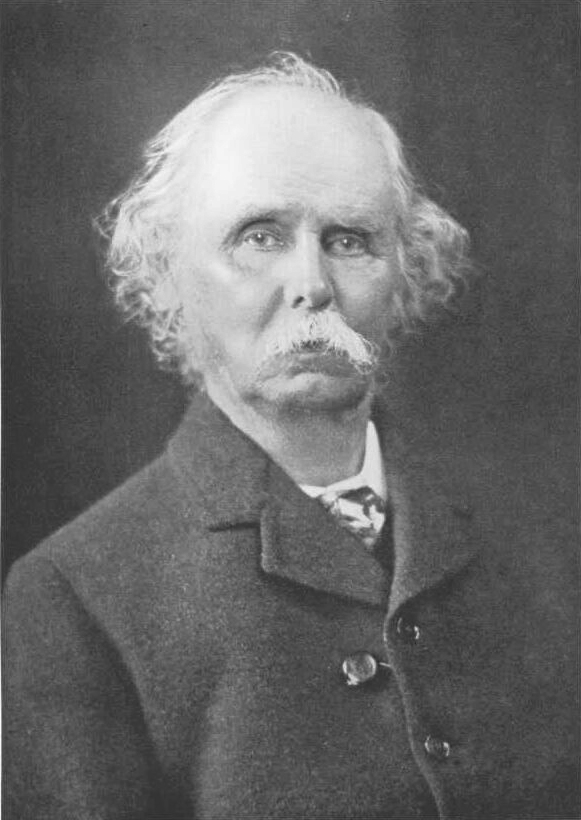
\includegraphics[width=0.5\linewidth]{img/ch0/Alfred_Marshall} \caption{Image Sourced from Wikipedia.}\label{fig:fig002}
\end{figure}

One of the founding fathers of modern economics, Alfred Marshall, writes in Chapter 1 of his Principles of Economics book:

\begin{quote}
``Political Economy or Economics is a study of mankind in the ordinary business of life; it examines that part of individual and social action which is most closely connected with the attainment and with the use of the material requisites of wellbeing.''
\end{quote}

The ordinary business of life: going to school, graduating, going to work, a career, dating and marrying, vacations, having children or not, the mortgage, car payments, illness, retirement, \ldots{}

All of these are parts of life for most of us, ordinary life.

\begin{figure}
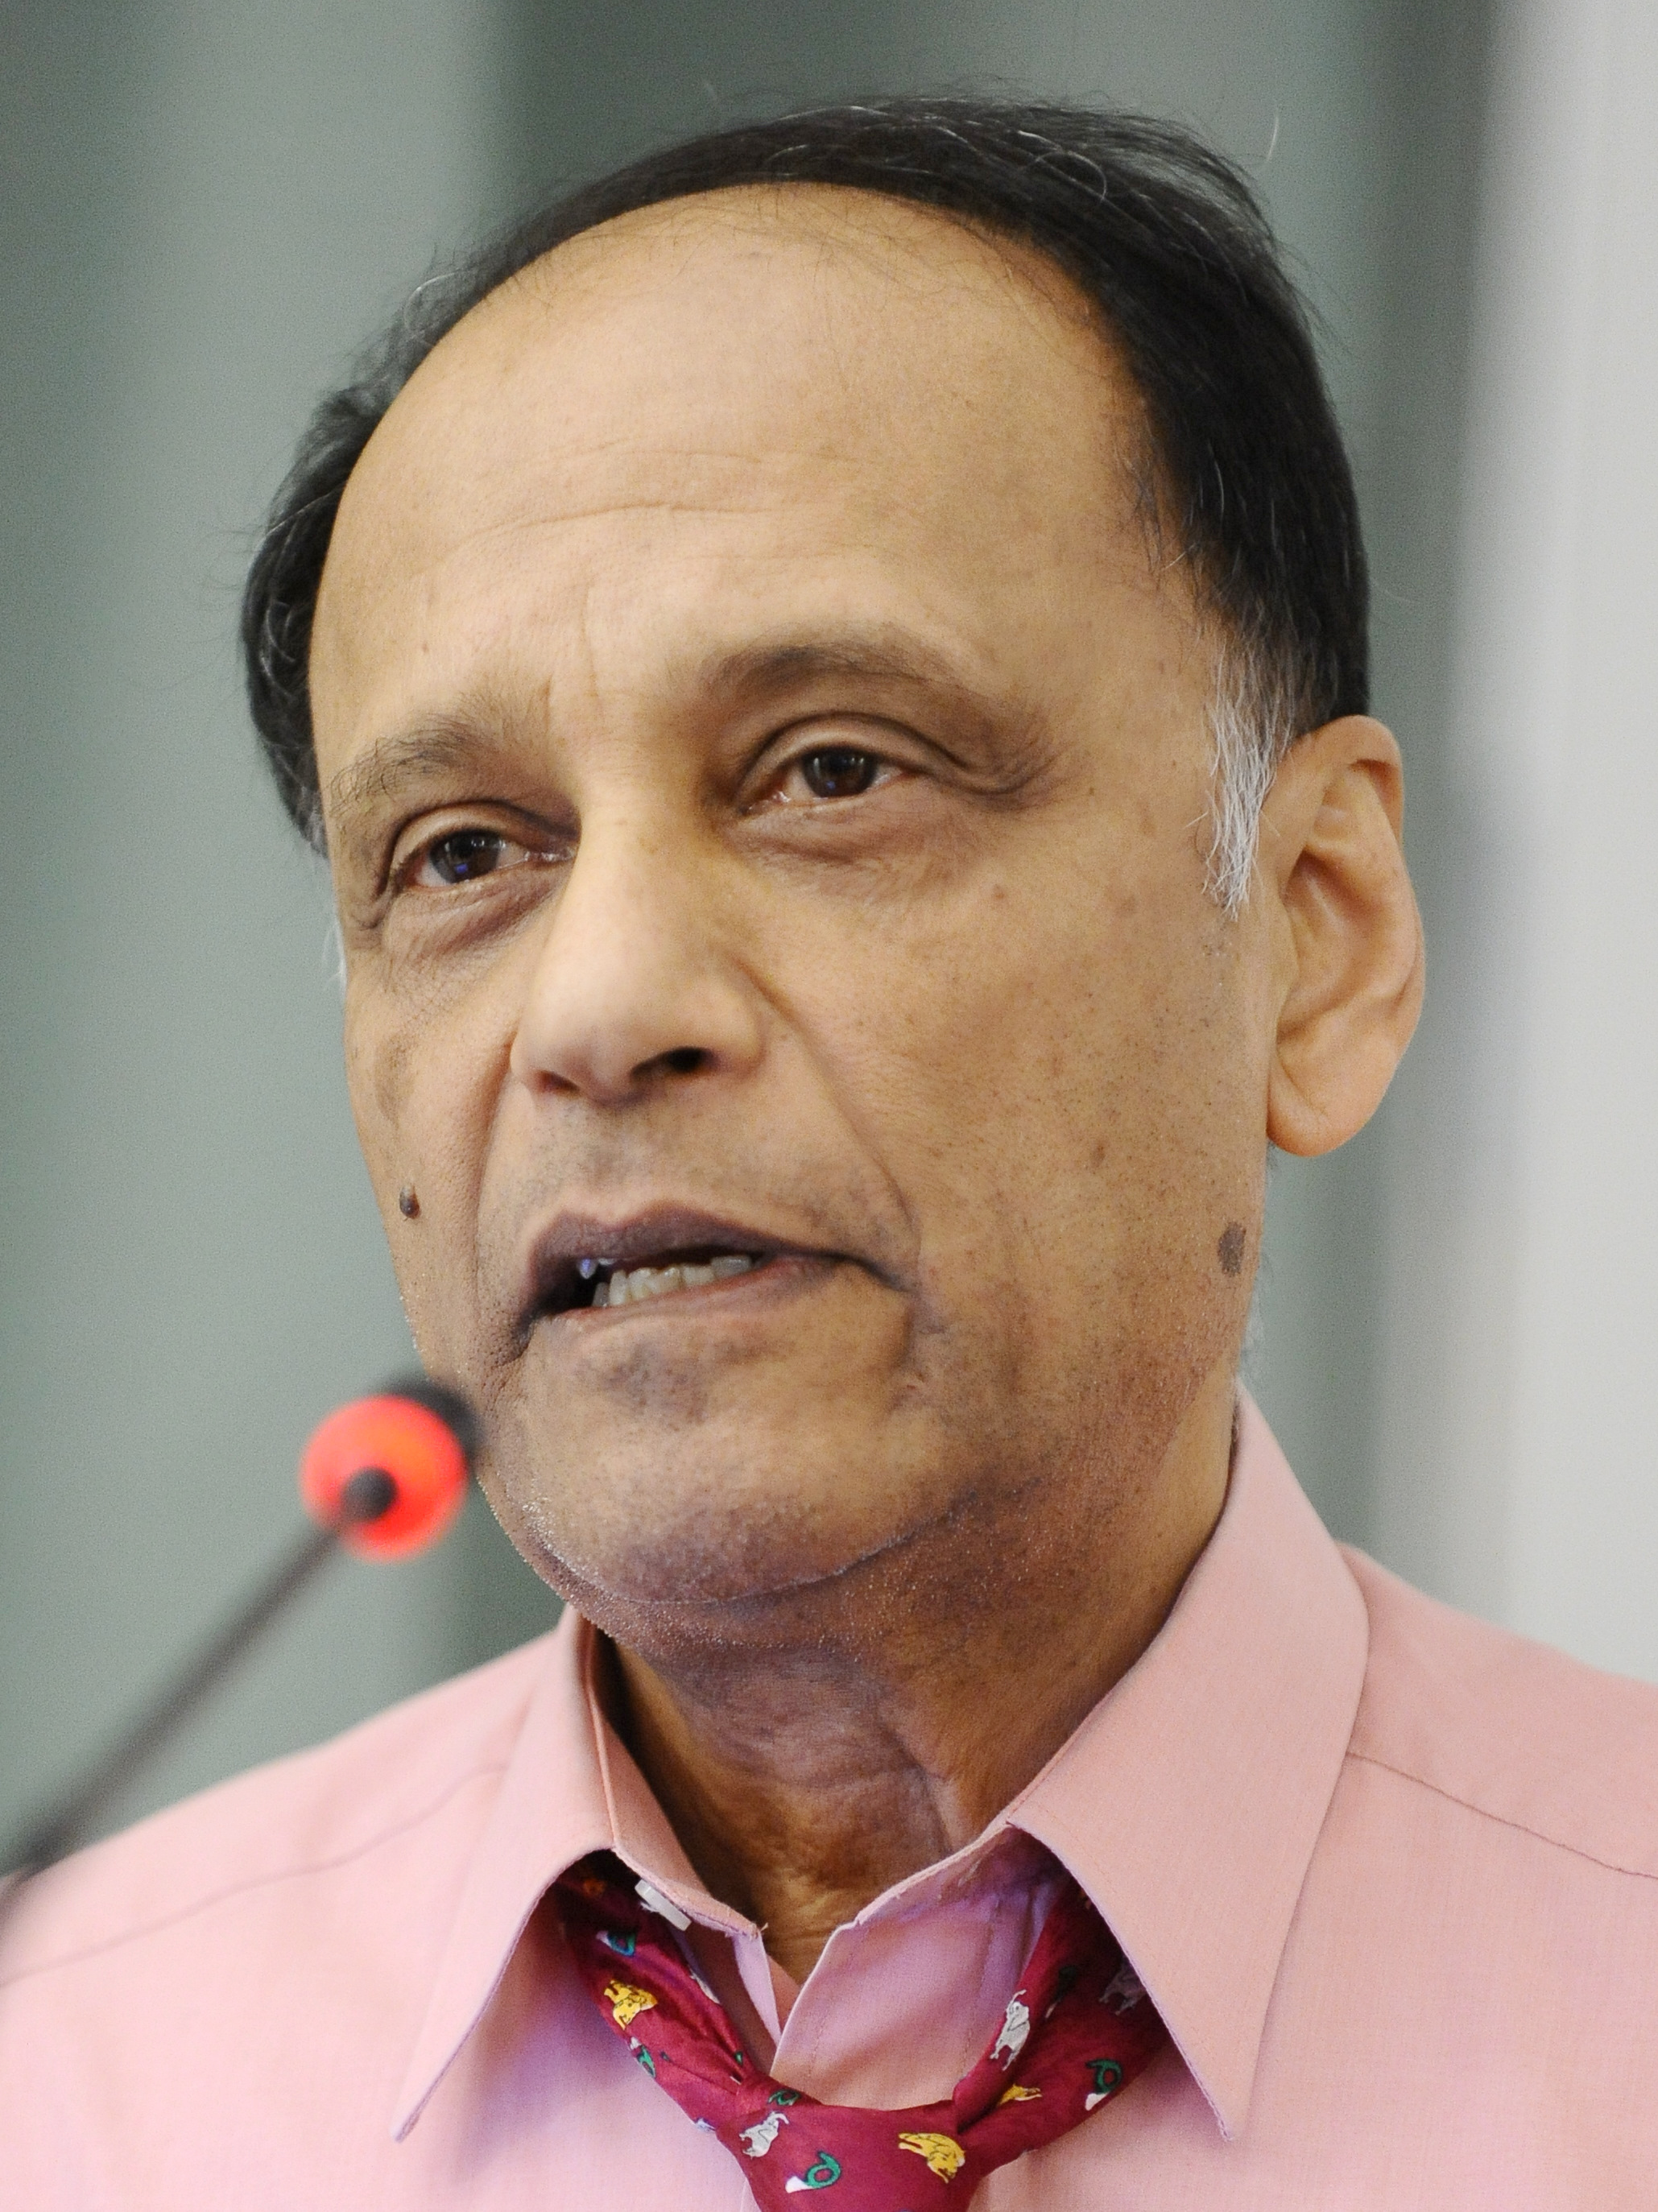
\includegraphics[width=0.5\linewidth]{img/ch0/Partha_Dasgupta} \caption{Image Sourced from Wikipedia.}\label{fig:fig003}
\end{figure}

One of the greats of modern economics, Partha Dasgupta\footnote{\url{http://www.econ.cam.ac.uk/people/emeritus/pd10000}}, writes

\begin{quote}
``These are no mere academic matters. If welfare and development economics, more generally political philosophy, are not about the circumstances in which people are born and the manner in which they are able to live and die, they are about nothing.''
\end{quote}

Evidently economics is about life from the moment we are born to the moment we die so anyway, with all its joys, with all its triumphs, but also with all its challenges, struggles, defeats and tragedies.

This includes the preemies that are born weighing less than 2 pounds with their and their parents' life - long struggle to flourish and to secure a comfortable life. How big are the medical bills? Does insurance cover them all?

\begin{figure}
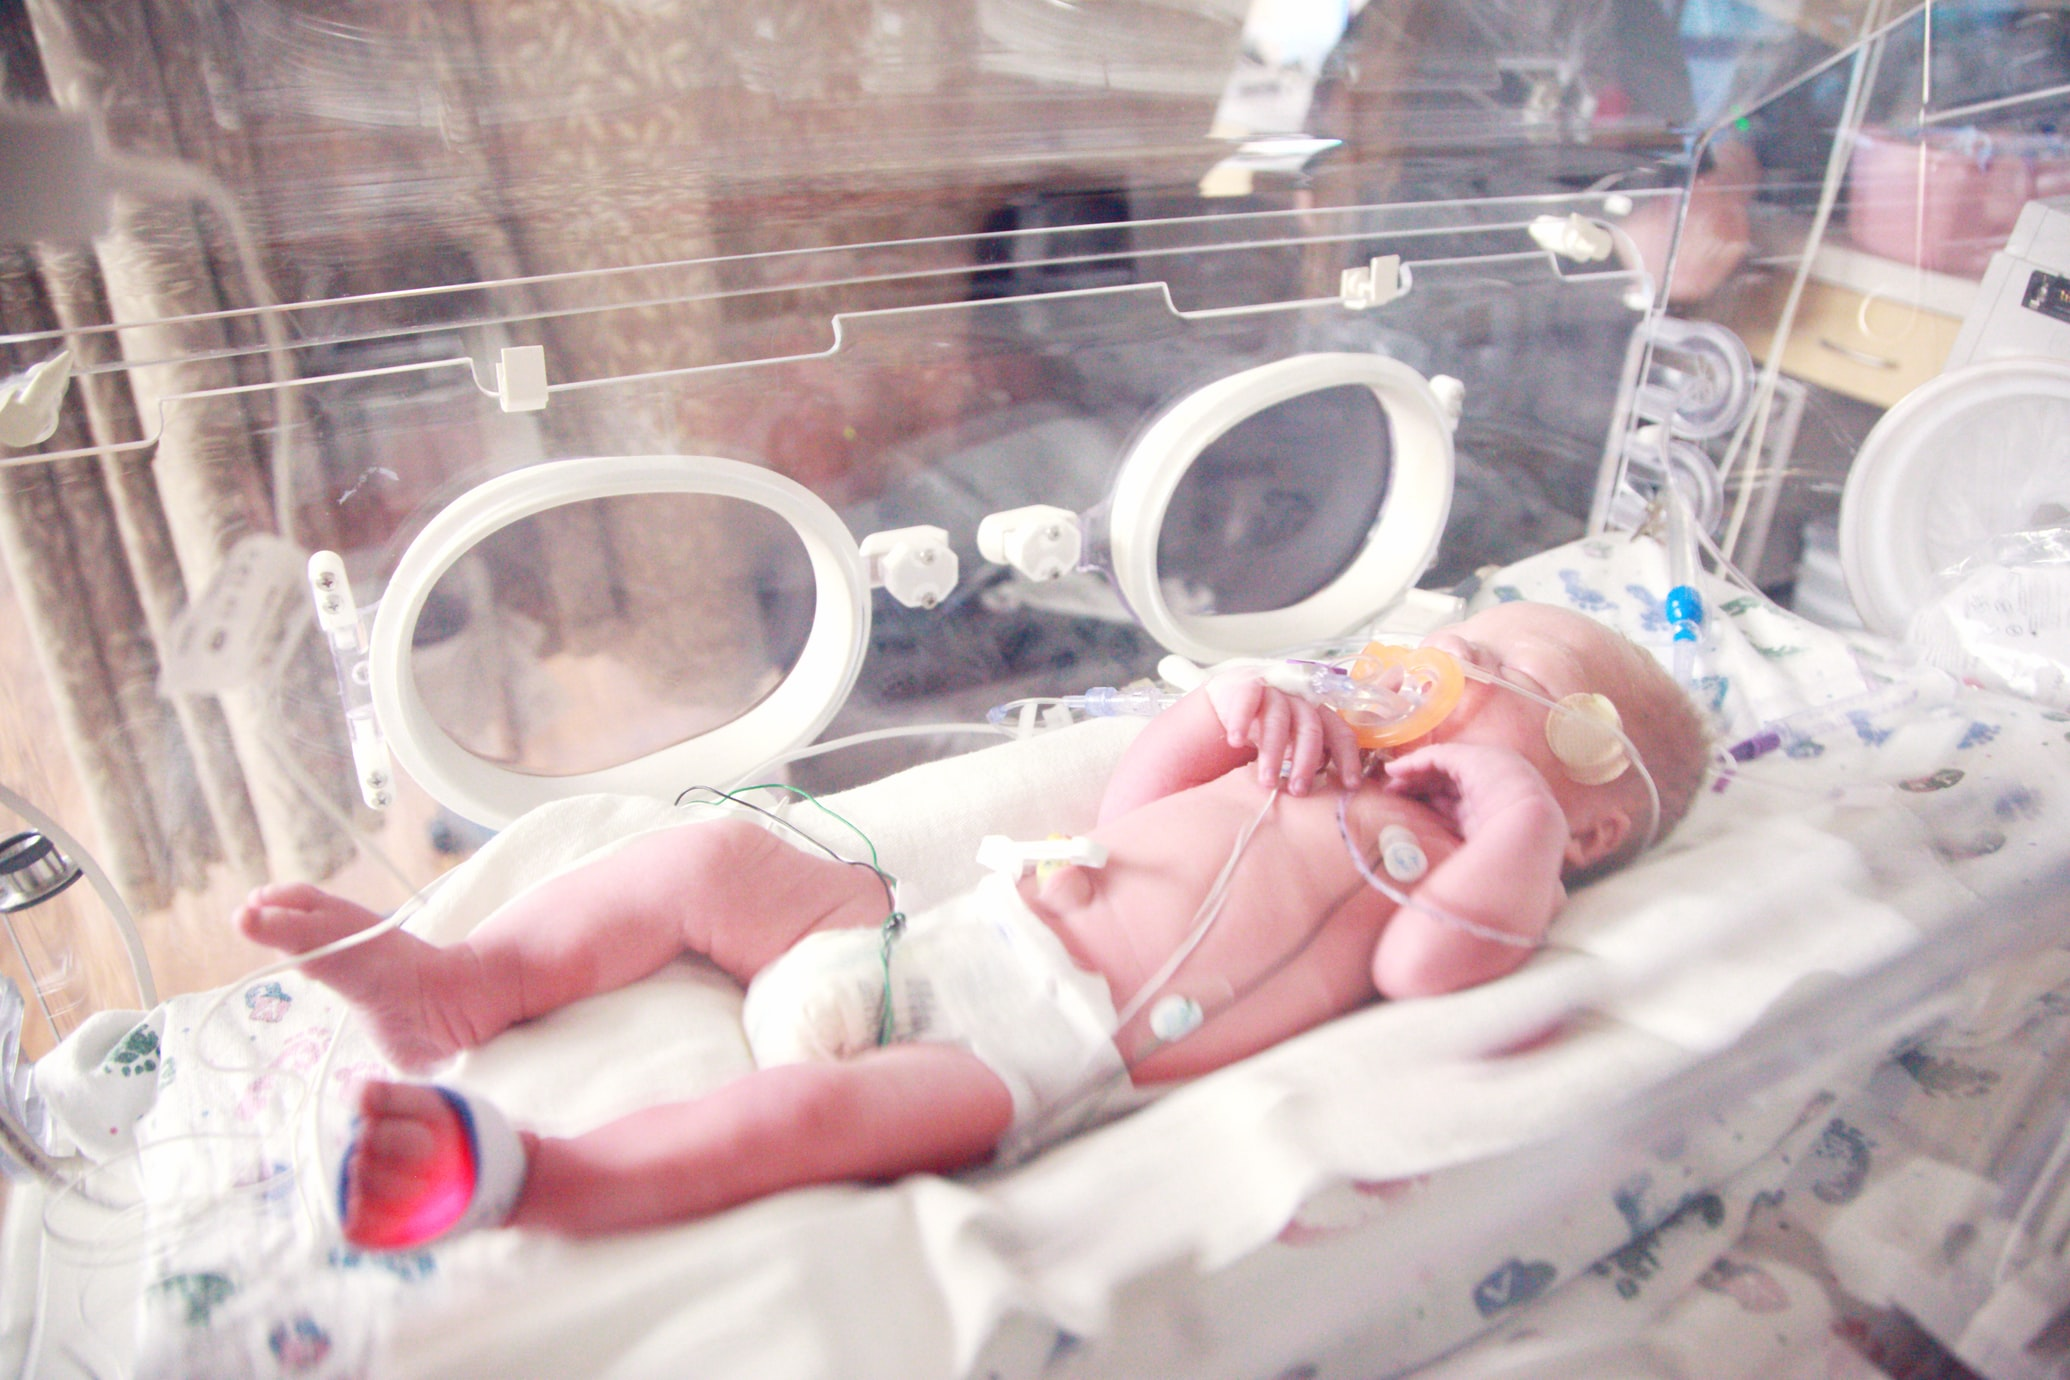
\includegraphics[width=0.5\linewidth]{img/ch0/fig4} \caption{Image Sourced from unsplash.}\label{fig:fig004}
\end{figure}

This includes the child born in the wrong ZIP code area that developmentally is already behind at age 3 and that will have a hard time catching up scholastically and that as a young adult will have difficulty making ends meet because of the poor employment prospects.\footnote{\url{https://research.upjohn.org/up_press/228/}}

This includes the young person who graduated from college with huge student debt that is impossible to be paid the back and that is very unlikely to be forgiven even in bankruptcy.

This includes the parents of young children who are torn between going to work to pay the bills and staying home with their children because there is no reliable and safe childcare during covid-19.

\begin{figure}

\includegraphics[width=0.5\linewidth]{img/ch0/fig5} \caption{Image Sourced from unsplash.}\label{fig:fig005}
\end{figure}

This includes the retired college professor whose physician tells him:

\begin{quote}
``Walter, with your lung cancer you have 6 months to live, on the outside. Now is the time to do the things you've always wanted to do but have never done'\,'
\end{quote}

But who, the following morning, gets ready to go to his office, and when reminded by his wife of the physician's advice that now is the time to do the things he always wanted to do, replies:

\begin{quote}
``That is exactly what I'm doing. I am doing what I've always wanted to do. I am going to the office to do my work.'\,'
\end{quote}

This includes the mother from Nicaragua, Guatemala, or Honduras, who flees with her children north, to what she thinks is a safer place for her children knowing full well the meaning and implications for her of the term ``cuerpomatic'\,'\footnote{\url{https://www.americasquarterly.org/blog/rape-another-threat-on-migrant-womens-journey-north/}}.

This includes things like ``positive assortative mating'' or ``like marries like''. Tall men/women tend to marry tall women/men. Another way of saying this is: The height of married couples is positively correlated. Highly educated women/men marry highly educated men/women. The level of education of married couples is positively correlated. It was not always like this.

This includes all those people who suffer from kidney failure, who are waiting for a transplant kidney, who may or may not get one. In this country, about 13 people die per day, because there are no transplants available.

\begin{figure}

\includegraphics[width=0.5\linewidth]{img/ch0/fig6} \caption{Image Sourced from unsplash.}\label{fig:fig006}
\end{figure}

Most textbooks define economics to be the study of the allocation scarce resources. A resource here is simply a means, something that is useful. Useful for a purpose. We usually assume that people have goals and that they will try to achieve these goals. But there are constraints that stand in the way.

Money is resource that allows us to buy stuff. For most of us money is scarce, our budgets are limited. Therefore, we must make choices. The fancy car or a super vacation? Paying the utility bill or paying the medical bill? A fancy wedding or a dream house?\footnote{\url{https://www.netflix.com/title/81113929}}

Time, perhaps our most valuable resource, is also scarce. You will surely notice this, as many have before you, during finals week. You will wish that there were five or six extra hours in each day.

Bandwidth, our ability to compute, to calculate, to process information, to decide rationally, is surely limited and many of us wish that our bandwidth were much, much bigger.

\begin{figure}

\includegraphics[width=0.5\linewidth]{img/ch0/fig7} \caption{Image Sourced from unsplash.}\label{fig:fig007}
\end{figure}

\hypertarget{what-is-economics-good-for}{%
\section{What is Economics Good For?}\label{what-is-economics-good-for}}

First and foremost, since economics is a social science, we would expect economics to be good and useful in explaining behavior. When we look around, there are all kinds of interesting observations that we would like to explain. And economics can help us go a long way towards providing explanations for all kinds of behavior.

\begin{enumerate}
\def\labelenumi{\arabic{enumi}.}
\tightlist
\item
  Why did grocery stores run out of toilet paper at the beginning of the covid-19 epidemic?
\item
  Why did women suffer more than men from the covid-19 induced epidemic when normally in other recessions men tend to suffer more employment losses than women?\\
\item
  Why are Dutch women taller than American women?
\item
  Why do women when they buy a house from a man pay a higher price than a man and when they sell a house to a man they get a lower price than a man?
\item
  Why did the price of bicycles rise during the covid-19 recession?
\item
  Why did the price off used cars rise during the covid-19 recession?
\item
  Why has the labor force participation of males been dropping for the last 20 or so years?
\end{enumerate}

The question is always:
Why? Why? Why?

Perhaps we can spend a little bit of time thinking about the following three examples of observations and ask why did these things happen?

In Maine in the 1800 Lobster was used commonly to feed prisoners and it was used commonly for fertilizer on the fields. Why?

In a recent 5K race in Bloomington Indiana there were participants in basically all age groups from age 16 all the way up to age 80. this was true for both men and women with one exception. in the category Between age 30 and 35 there was not a single female participant. Why?

According to some reports from field workers In a refugee camp for the Rohingya in Bangladesh There were children older than five years of age and younger than 2 but there were no children between the ages of 2 and 5. Why?

We will see how economics can provide answers too many of these why? why? why? Questions.

Economics can also provide answers to questions like what are the underlying assumptions that some individuals make under which their behavior might be rational?

If we consider a CEO who believes they are running late to a meeting for a merger worth millions of dollars. We might think driving at very high speed under these circumstances actually makes a lot of sense. It is the rational thing to do.

On May 25, 2020, Amy Cooper, a white woman, let her dog off its leash in Central Park. Christian Cooper, a black male who was in the park watching birds asked her to leash her dog back up. Amy Cooper called the police alleging an ``African American man'' was threatening her. \footnote{\url{https://www.nytimes.com/2020/07/06/nyregion/amy-cooper-false-report-charge.html}}

Under what assumptions is the behavior of Amy Cooper in Central Park rational? \href{https://www.ncronline.org/news/opinion/assumptions-white-privilege-and-what-we-can-do-about-it}{This article} digs into this. Rationality here and in the rest of these notes means: Our actions are guided by a particular purpose or goal, taking into consideration all constraints and all relevant information. Bryan Massingale in the article below list many assumptions under which Amy Cooper's behavior in Central Park is actually rational. Her actions seem to make sense under the assumption that her word as a white female would have more weight than the word off a black male. Since she must have thought that any police officers, not a particular police officer, summoned by her would give more credibility to her word than to the black male, she must have believed and hoped for what we would call systemic racism. Her actions make sense, her actions are rational, if she believes in systemic racism.

The second thing economics is good for is to evaluate policies. Policies are just the things governments, in particular, and institutions in general do. The federal government determines spending on defense and Medicare. It regulates immigration to this country. The state government chooses educational policies and whether to legalize weed. A local government decides to fund public parks and bicycle paths. A country club determines the rules for the use of a golf course. A faith organization chooses particular youth programs. A corporation chooses particular HR policies.

In each one of these cases we want to know:

\begin{itemize}
\tightlist
\item
  Does the policy work?
\item
  Is it a good policy?
\end{itemize}

We want to be able to hold public officials accountable for the policies they pick. In order to be able to do, we need to be able to figure out how people respond and react to these policies.

This leads us to a subject that is covered in the opening chapters of all introductory economics textbooks:

\textbf{The law of unintended consequence}

The law of unintended consequences simply states that when a policy is changed, people will respond to that policy change, and frequently in ways that are difficult to forecast by the policy maker. Of course, the more careful the policy maker thinks about possible responses of people to the change in the policy, the fewer surprise responses to the policy there will be. But it is a testimony to human ingenuity and creativity that even with the best intention the best laid plans of mice and men often lead to disastrous outcomes. My guess is that such adverse responses to policy changes will never be eliminated, even after the most careful analysis of the proposed policy change.

It should not be a surprise that bad people will respond to changes in a policy. People simply do what they believe is in their best interest and when incentives change, chances are their behavior will change as well.

If I announce that in my class there will be a final exam that is comprehensive, that is the hardest exam on campus with a pass rate off only 30\%, there are a variety of possible reactions to this kind of an announcement. Some students will decide to study harder, some students might get a tutor, some students might decide to come to office hours more frequently. Some students might just give up, drop the class and wait until that class is offered by a different faculty member who has easier exams. This is just incentives at work. But we have to acknowledge that the different students will respond in different ways and it is just extremely difficult to predict the behavioral response a particular student.

There are some interesting responses to changes in government policy.

\hypertarget{examples}{%
\subsection{Examples}\label{examples}}

\begin{enumerate}
\def\labelenumi{\arabic{enumi}.}
\tightlist
\item
  \textbf{(Epidemics I)} I heard of a convenience store in Virginia that had attached to it a video arcade with a separate entrance. During covid-19, the convenience store was declared essential and allowed to stay open, the video arcade shut by order of the government. How did the owner of the convenience store and the video arcade respond to this government policy? He simply moved some of the video games into the convenience store, thereby increasing the density of customers in the store and the therefore the risk of infection of customers. \textbf{NEED CITATION}
\end{enumerate}

\begin{enumerate}
\def\labelenumi{\arabic{enumi}.}
\setcounter{enumi}{1}
\tightlist
\item
  \textbf{(Epidemics II)} \footnote{\url{https://crofsblogs.typepad.com/h5n1/2020/05/trumps-europe-travel-ban-triggered-covid-19-spreadin-the-us.html}} On March 11, 2020, President Trump announced a travel ban from most countries in Europe to be effective March 13th and to last 30 days. If you are an American traveler in Europe, how would you respond to this announcement? If you are an American tourist in Europe, how would you respond? If you are an American on business in Europe, how would you respond? Or, if you are an American student on an exchange program in the affected European countries, how would you respond? Regardless of your original plans for your return trip, you might well conclude that the best course of action for you is to hightail it home as quickly as you possibly can. Evidently, many Americans decided that this was indeed their best course of action, so they change their plans and return home as quickly as possible. As a consequence, American airports on March 12 and 13 were overcrowded, contributing to the further spread of the virus. Perhaps this crowding might have been avoided to some degree buy more carefully planning the return flights and spreading out over time the arrival of these flights into international American airports.
\end{enumerate}

\begin{enumerate}
\def\labelenumi{\arabic{enumi}.}
\setcounter{enumi}{2}
\tightlist
\item
  \textbf{(Work Incentives)} During the financial crisis off 2008 and 09 the governments in many affected countries designed rescue packages to bailout banks, at least the largest banks. Some of these rescue packages contain explicit caps on bonuses for banking executives. If the government imposes caps on those bonuses, how might banks respond to such limitations? Well, if I cannot reward my employees through higher bonuses, I can still reward my employees by increasing their base salaries. To the extent that the bonuses are used to reward exceptionally good performance and thereby provide incentives for such exceptionally good performance, this cap on bonuses seems to have one adverse effect: weaker incentives for exceptional performance. Not sure if that is what you want.
\end{enumerate}

\begin{enumerate}
\def\labelenumi{\arabic{enumi}.}
\setcounter{enumi}{3}
\tightlist
\item
  \textbf{(Health)} Imagine you are concerned with excessively long waiting times at emergency rooms in the hospitals in your state. Suppose you want to design a scheme that rewards hospitals to decrease those waiting times. So, you collect the data on average waiting times in these emergency rooms and then you design rewards for those hospitals who reduce the waiting times the most. If you measure waiting time from the moment the patient comes through the door to the time the patient is treated, how might hospitals actually respond to this new policy?
  Hospitals might ask the ambulances to wait in the hospital parking lot. Surely this is not a desired outcome.
\end{enumerate}

\begin{enumerate}
\def\labelenumi{\arabic{enumi}.}
\setcounter{enumi}{4}
\tightlist
\item
  \textbf{(Education)} Supposed you want to reward teachers for better performance of their students on standardized tests. Suppose the stakes, the rewards are big. How might the teachers respond to these incentives? Surely there are many possibilities.
  Some teachers might better prepare their lessons.
  Some teachers might spend more time with students who are struggling.
  But some teachers might also provide caffeinated sugary drinks to their students the day of the test to get a short time boost in attention and concentration to improve their performance. I suspect the dentists will love this.
  Or, and this is an extreme case, some teachers might actually be induced to cheat on behalf of their students. One example of teachers engaging in such cheating is documented in the first book Freakonomics. \textbf{NEED CITATION}
\end{enumerate}

\begin{enumerate}
\def\labelenumi{\arabic{enumi}.}
\setcounter{enumi}{5}
\tightlist
\item
  \textbf{(Gender)} \footnote{\url{http://ftp.iza.org/dp9904.pdf}} Family leave policies are intended to allow moms and dads to spend quality time with their new-born babies. In many places/organizations there has been a gradual shift from no leave, paid or unpaid, to maternity leave for the mom to family leave for both mom and dad, when a baby is born. In some organizations there is still no maternity or family leave policy in place and women have to take sick days or personal days to deliver their baby. At a typical university maternity or family leave is ties to ``stopping the tenure clock''. Stopping the tenure clock simply means, that mom and/or dad have extra time, often one year, to be considered for tenure. Tenure basically ensures lifetime job security. Its is a BIG deal.
  Allowing dads time off and stopping the tenure clock for dads as well as for moms is often seen as a great equalizer of men and women, dads and moms. After all, now dad can spend time with his baby as well. What could possibly be or go wrong with that?
  The paper below shows that the policy of providing gender neutral family leave and stopping the tenure clock in a gender-neutral way, increases dad's chances of tenure by 19 percentage points and decreases mom's tenure of tenure by 22 percentage points.
  So much for achieving gender neutrality!
\end{enumerate}

\begin{enumerate}
\def\labelenumi{\arabic{enumi}.}
\setcounter{enumi}{6}
\tightlist
\item
  \textbf{(Gender)} \footnote{\url{https://www.cesifo.org/en/publikationen/2020/working-paper/caught-between-cultures-unintended-consequences-improving}} The German government passes a law that grants automatic German citizenship tights to all immigrant children born in Germany after January 1, 2000. You might think that such a law would benefit all immigrants regardless of country of origin, skin color, religion, sex, gender identity and age. Why? It is just a right. The law increases the realm of the possible. It increases opportunities. It does not take away any opportunities. What could possibly be wrong with more choices, more opportunities? So, one would be inclined to think that all immigrants would be better off and report being happier. And in that believe we would be wrong. Why? The law of unintended consequences strikes again.
  Self-reported happiness declined after this law was passed for Muslim girls. Muslim immigrant girls become disillusioned. Muslim parents are less likely to help their daughters who qualify for citizenship with their homework. They are also less likely to speak German with their daughters. Muslim immigrant girls who qualify for German citizenship are less likely to self-identify as German.
  The law of unintended consequences truly rears its ugly head.
  None of these effects are found for Muslim boys. None of these effects are found for children of other faiths.
  Why do we find these effects for Muslim immigrant girls? Parents of Muslim immigrant girls react strongly to counter effect the pull of German society to keep their daughters withing their cultural and religious traditions.
\end{enumerate}

\hypertarget{exercises}{%
\subsection{Exercises}\label{exercises}}

\begin{enumerate}
\def\labelenumi{\arabic{enumi}.}
\tightlist
\item
  Suppose the State passes a law that allows for ``No knock warrants''. \href{https://en.wikipedia.org/wiki/No-knock_warrant\#:~:text=In\%20the\%20United\%20States\%2C\%20a,knocking\%20or\%20ringing\%20a\%20doorbell}{See here} if you are unsure what this is.
\end{enumerate}

Make a list of the possible ``unintended consequences'' of this policy.

Who would get impacted by this policy? Positively or negatively?

How hard is it to foresee/forecast these consequences?

\begin{enumerate}
\def\labelenumi{\arabic{enumi}.}
\setcounter{enumi}{1}
\tightlist
\item
  President Trump issued an Executive order on June 22, 2020 to severely limit H1-B and L1 visas. H1-B visas are visas issued so American companies can hire high-skilled immigrants. L1 visas allow American multinational corporations to transfer foreign managers and employees to their offices in the US. \footnote{\url{https://www.nber.org/papers/w27997}}
\end{enumerate}

Make a list of all the effects of this policy. Who would get impacted by this policy? Positively or negatively?

How hard is it to foresee/forecast these consequences?

\hypertarget{role-of-theory}{%
\section{Role of Theory}\label{role-of-theory}}

What is the role of theory in economics?

A quote by a 12th century philosopher, Peter Abelard:

\begin{quote}
``The man of understanding is he who has the ability to grasp and ponder the hidden causes of things. By hidden causes we mean those from which things originate, and these are to be investigated more by reason than by sensory experiences.''
\end{quote}

We can paraphrase this by saying: If we want to understand stuff, we ought to rely more on our brain and think more about how things might actually work, rather than collecting data with our senses.
Charles Darwin, in a letter to one of his friends expressed a similar opinion:

\begin{quote}
``About thirty years ago there was much talk that geologists ought only to observe and not theorise; and I well remember someone saying that at this rate a man might as well go into a gravel-pit and count the pebbles and describe the colors. How odd it is that anyone should not see that all observation must be for or against some view if it is to be of any service!''
\end{quote}

I interpret that last clause in Darwin's letter to mean: All observations must be used to either confirm or reject a hypothesis or theory, if the observation is to be of any use at all. That implies that theory comes first.

So, what is this thing called a ``theory''? I will use the words: theory, model, and abstraction as synonymous. A theory is a creation of our minds; it is an idea of how some part of the word operates or might operate.

The theories we use will be different in economics and in physics. Even within economics there will be different theories or models. Macroeconomists will use different models than economists who study anti-trust. The main job of a model is to help us understand how a part of the world works. Any theory or model is supposed to be useful, for understanding.

\hypertarget{abstractions}{%
\subsection{Abstractions}\label{abstractions}}

How is an abstraction useful? Suppose the job is to drive from Indianapolis, IN to Columbus, OH. We need a map to help us get there.

\newpage{}

Above we have a map. It has all kinds of information. The IN-KY border. If we zoom in, there are many roads, many cities. Zoom out, there is Lake Michigan, Lake Erie. A whole bunch of information about Illinois. Much of this information is not relevant if the task is to get from Indianapolis to Columbus.

In order to get from Indy to Columbus, not much information is needed. Most, practically all of the information above is useless and needs to be discarded. Pretty much the only information needed is illustrated below. All we need is the starting point, Indy, the endpoint, and the instructions to get on I -70 in Indy until the sign ``Columbus, OH'' appears. This is really all that is essential.

INDY---------------------------I 70---------------------------------Col

There are a few more things that one might reasonably add to our ``model'' of the relevant piece of geography. It might be useful where the gas stations are, especially the ones with clean bathrooms, and where the coffee shops are so the driver does not fall asleep. One such establishment, marked by G for gas station, is added in the model below.

INDY---------------------------I 70--------------------G-----------Col

\hypertarget{prejudice-based-wage-discrimination}{%
\subsection{Prejudice-Based Wage Discrimination}\label{prejudice-based-wage-discrimination}}

How to find prejudice-based wage discrimination?

In this example I will try to show that economic theory can generate useful insights or knowledge. The way this works in this example is that economic theory will suggest precisely where we have to look for evidence. The issue or example that we will use here is the question:
How, if, and to what extent does racial prejudice show up in or generate wage discrimination by race?

The work in economics on racial discrimination goes back at least to the seminal work by Nobel Laureate Gary Becker from the University of Chicago.

For starters, we have to distinguish between prejudice and wage discrimination. Prejudice is an attitude, a negative attitude, a sentiment toward a particular group of people, Blacks for example. Wage discrimination is a particular outcome in labor markets that simply says comparable blacks and comparable whites earn different wage rates.
The question then is: How, to what extent, if at all, does racial prejudice determine such wage discrimination?

In order to start thinking about this issue, we will consider a very simple example. Blacks make up about 10\% off the population or the labor force. There are two distinct labor markets. In labor market 1 the population of white people exhibits basically no racial prejudice. In labor market 2, the population of white people exhibits very strong racial prejudices.

In which labor market would we expect wage discrimination by race to be strongest? Labor market 1 or labor market 2?

Without a moment's thought most of us would be tempted to say: Of course, racial discrimination higher, stronger, worse in labor market 2 than in labor market 1.

But that would be missing an element off the story that probably is very important.

Blacks will most likely know or at least have some pretty good information on where the racists live, in which labor market they operate. Why would they know this? Chances are they have experienced the manifestations of racism and through their social network this information is broadly shared.

So, to the extent that blacks have information on manifestations of racism and to the extent that they are free to move between labor markets, to choose their place of employment, they will probably move from labor market 2 two labor market 1. This is of course, holding other things equal. holding other things equal just means that in all other aspects these two labor markets are roughly comparable. they only differ in this one aspect: prejudice.

So, if blacks can move freely, relatively freely, they will choose labor market 1 over labor market 2 in which case there might be very little racial wage discrimination in labor market 2. If all Blacks where to move into labor market one, then there would be no racial wage discrimination in labor market 2 at all.

Therefore, our answer that labor market 2 will exhibit more wage discrimination than labor market 1 is probably false.

There is a \href{https://papers.ssrn.com/sol3/papers.cfm?abstract_id=1073644}{recent paper linked here}, together with a \href{https://www.youtube.com/watch?v=N38XrQ6x7ck}{short video} by one of its authors, that uses currently available data to show us exactly where and how we should look for the impact of prejudice on labor market discrimination.

We start with constructing a racism distribution. This is not just some fancy Ivory Tower notion. This distribution is firmly grounded in data. There is a data set that is widely available, called The General Social Survey, GSS, that asks questions like:

\begin{itemize}
\tightlist
\item
  How would you respond if your daughter dated a black person?
\item
  Would you vote for a black man for president of the United States if he were qualified?
\end{itemize}

Answers to questions like these can be put together to create an index of racism and then a distribution of racism in a particular locality. The figure below illustrates such an example off a racism distribution.

Some researcher suggests that in order to assess the impact of prejudice on wage discrimination one should look at a correlation between the average or median degree of prejudice and the average level of wage discrimination. They collect the best data available for the 50 States and calculate or estimate that correlation. They find nothing.

Why?

Just like in the example with 2 labor markets, Blacks will, if they can, avoid the right tail of the racism distribution. They will shift to the left as far as possible in the racism distribution.

In Wisconsin, about 6\% of the labor force is black. If they all seek employment, they would be matched with some, mostly likely white, employer. If we line up all white employers on a racism distribution, with the least racist employers on the left and the most racist employers on the right, then black workers would seek employment as far away from the most racist employers as possible. Black workers would go to the left of the racism distribution as much as possible. Since Blacks in Wisconsin make up 6 percent of the population, these 6 percent would then be seeking employment from the 6 percent of the least racist employers. Since Blacks are seeking employment as far to the left tail of the prejudice distribution as possible, then it is the 6percentile of the prejudice distribution that matters for wage discrimination. Not the average, not the median. The 6 percentile.

In Mississippi, about 34\% of the labor force is black. In Mississippi, wage discrimination is determined by the 34th percentile of the prejudice distribution. Not the average, not the median, not the 6th percentile. The 34th percentile.

\textbf{STATISTIC FUNDAMENTALS - WHAT IS A PERCENTILE}

So far, we have not looked at any data; so far this is all theory.
What is in the data?

When you look for the connection between prejudice and wage discrimination by looking at averages you find nothing.

But when you look for it in the way suggested by the theory, the 6th percentile of prejudice distribution in WI, the 34th percentile in MS, then BINGO! There it is, clear and significant evidence linking prejudice to wage discrimination. You just need to know where to look. Theory helps.

\hypertarget{dealing-with-data}{%
\section{Dealing with Data}\label{dealing-with-data}}

\hypertarget{empirical-regularities}{%
\subsection{Empirical regularities}\label{empirical-regularities}}

First of all, we note that we are more interested in empirical regularities than in singular observations. Jennifer is 5'4'' is an example of a singular observation. That is only one observation. Dutch women are tall is an example of an empirical regularity. This observation is more general. We would find this if we looked at a sample of women from Amsterdam, from Rotterdam, from The Hague, etc.

Rich people live longer than poor people.

This is a fact, in Indiana, New Jersey and in Kentucky. It is also true in France and in Japan.\footnote{\url{http://www.equality-of-opportunity.org/assets/documents/healthineq_summary.pdf}}

The sex ratio in the US is 1.04. The sex ratio is the ratio of the number of women to the number of men. For each 100 men in this country there are 104 women. If you look up this ration by State, there is some variation. For most states, there are more women than men. But there are exceptions. In some Western states, there are more men than women. These exceptional states include Alaska, Montana, Wyoming. You may want to ask why there are such large differences in sex ratios across the 50 States.

Numbers: Big or small?

One of the important issues we have to discuss is: Are numbers big or small. This is especially true when we are talking about dollars, taxes, expenditures, the size of government programs.

\hypertarget{examples-1}{%
\subsubsection{Examples}\label{examples-1}}

\begin{enumerate}
\def\labelenumi{\arabic{enumi}.}
\tightlist
\item
  After the Haiti earthquake in 2010, the US government committed \$100 million in earthquake relief. Big number, small number? It might look like a big number. But when you consider that there are over 300 million Americans, we realize that each of us gave about 30 cents, which looks miserly. Of course, this does not include private charitable contributions.
\end{enumerate}

\begin{enumerate}
\def\labelenumi{\arabic{enumi}.}
\setcounter{enumi}{1}
\tightlist
\item
  The cost of the Apollo mission which ultimately landed a man on the moon has been estimated to be about \$150 billion, in 2019 dollars. In 2019 the White House made a request to combat deaths from illicit opioid abuse to the tune of \$7 billion. In 2018 over 67,000 people dies from opioid overdoses. Is \$7 billion a big number or a small number?\footnote{\url{https://www.whitehouse.gov/briefings-statements/white-house-seeks-billions-record-investments-stop-drug-epidemic/}}
\end{enumerate}

\begin{enumerate}
\def\labelenumi{\arabic{enumi}.}
\setcounter{enumi}{2}
\item
  According to an article in The Economist, August 8 -14, 2020 world- wide spending on research for a Covid-19 vaccine was about \$10 billion. Sure sounds like a heck of a lot of money. But. Just in the US, the number of people who have died, at that time, was about 100,000. The value of a statistical life\footnote{Kip Viscusi \url{https://law.vanderbilt.edu/bio/w-kip-viscusi} pioneered the research on the value of a statistical life.} in the US for the median age American is about \$10 million. Since Covid-19 takes mostly older people we might use \$5 million for the value of an older statistical life. The typical failure rate in late stages of vaccine trials is about 20\%. Multiplying the value of an older statistical life by the number of Americans who dies because of Covid-19 we get:

  \$100,000 \times 5 \times 1,000,000 = \$ 500 billion

  Covid-19 does not only kill Americans. And now we know that the death toll is much higher. Should we have spent more on vaccine research in 2020?
\end{enumerate}

\hypertarget{correlation-vs-causation}{%
\subsection{Correlation vs Causation}\label{correlation-vs-causation}}

This distinction is crucial. Knowing whether 2 variables are correlated is useful, but it is not enough. In order to make any kind of policy decision we must know causation. Correlation only tells us about a statistical relationship. Two variables may be positively correlated or they may be negatively correlated. Suppose variable X is positively correlated with variable Y. Then if X is large (small), then Y is large (small) as well. If the two variables X and Y are negatively correlated, that means that If X is large (small), then Y is small (large). Of course, there is also the possibility of no correlation.
My typical calorie intake is positively correlated with my body weight.
The time students spend studying for Finite Math exams may be negatively correlated with the grades in English classes.
Whether students are vegetarians or not is ( I suspect) not correlated with their grades in introductory History classes.
We can think of these correlations as patterns in the data. They tell us nothing about causation.

Causation is an altogether different story. Causation means that one event leads to another. The event ``An increase in the price of socks'', will lead to the event ``Gerhard buys fewer socks''. We will talk about this at some length in this class. The event ``90 percent of Americans getting the Covid-19 vaccine'' will lead to the event ``Americans achieve herd immunity''. The event ``Gerhard drives like a maniac on the interstates'' leads to the event ``The probability of fatal car crashes rises''.\\
There are lots and lots of examples like this. We need to be able to infer causality if we want to have any hope that the policies we pick actually make things better.

If two variables, X and Y, are positively correlated, there are several possibilities concerning causation:

\begin{enumerate}
\def\labelenumi{\arabic{enumi}.}
\tightlist
\item
  X could cause Y: an increase in X could cause an increase in Y. An improvement in nutrition in childhood causes an increase in adult height. There is no way adult height could influence the quality of childhood nutrition.
\item
  Y could cause X: an increase in Y could cause an increase in X.
\item
  X could cause Y AND Y could cause X: You study hard for your econ class and as a consequence you do well in the class. And: Since you do well in your econ class, you like econ and therefore you study harder. The hard part might be to find out which effect is stronger.
\item
  X does not cause Y, nor does Y cause X. But there is another variable, Z, that causes both X and Y.
\end{enumerate}

In order to tease causation out of the data, we try to create what we call \textbf{a parallel universe.}

The point of this parallel universe is to look at two cases, two ``universes'' that are equal in all aspects except one aspect, the aspect we want to study.

\hypertarget{examples-2}{%
\subsubsection{Examples}\label{examples-2}}

\begin{enumerate}
\def\labelenumi{\arabic{enumi}.}
\item
  Suppose I want to study the effect of the Florida ``stand your ground law'' on homicides in Florida. Then I will collect all kinds of data for Florida. And I will collect the same kind of data in similar states. It would make little sense to compare Florida to Norway. But comparing Florida to states with similar income distribution, similar ethnic composition, similar poverty rates, similar age distribution makes sense. Like Georgia, Alabama, Arkansas.

  Then we can compare homicide rates in Florida to those in other states that did not pass stand your ground laws. That is one difference we can exploit for our analysis. The other difference we can exploit for our analysis is to what happened to the trend in homicides before and after the law was passed.

  The conclusion that emerges in this case is quite shocking: It appears that the stand your ground law has caused an INCREASE in homicides.\footnote{\url{https://jamanetwork.com/journals/jamainternalmedicine/fullarticle/2582988}
    For more comprehensive evidence, see
    \url{https://www.rand.org/research/gun-policy/analysis/stand-your-ground/violent-crime.html}}
\end{enumerate}

\begin{enumerate}
\def\labelenumi{\arabic{enumi}.}
\setcounter{enumi}{1}
\tightlist
\item
  In example 6 of the Law of Unintended Consequences above, how could the researchers ``establish'' or ``find'' a parallel universe? Sometimes you are just lucky. The law applied to all immigrant children born after January 1, 2000. The law separates those immigrant children born before that date from those born after that date. Children borne 6 months before and children borne 6 months after will be in the same school grade. They will be very, very similar in all or at least most other aspects. The fact that the law kicks in January 1 is very fortuitous for researchers. It creates almost ideal conditions to have a treatment group and a control group. Having a treatment group and an identical control group is what we mean by having ``a parallel universe''.
\end{enumerate}

\begin{enumerate}
\def\labelenumi{\arabic{enumi}.}
\setcounter{enumi}{2}
\item
  In 2015, the City of Chicago banned all single use plastic shopping bags that were less than 2.25 mils thick. All other bags were unregulated. What are the consequences of this ban?

  Short answer: Stores responded by using bags that are still made of plastic and that are thicker and therefore use MORE plastic. Another unintended consequence.

  Unintended consequences seem to be everywhere.

  How would we know? How can we infer causality? Where are the parallel universes? Where are treatment and control groups?

  The researchers reasoned that stores just inside city limits ought to be very similar to store just outside if city limits in the suburbs. The researchers also reasoned that shoppers just inside the city limit are very similar to shoppers just outside the city limit. So, data from just outside the city limit can serve as a parallel universe to what is going on inside the city limit.

  There is more: Stores and shoppers just before the ban and just after the ban are going to be very similar. So, in addition to the comparison of inside and outside the city limit we have the comparison of just before and just after the ban. Looking at these two comparisons allows the researchers to nail down the effect of the ban: Disposable bag use remained very high. Many grocery stores just used bags that were just thick enough to be above the limit.\footnote{\url{https://www.nber.org/papers/w28499}}
\item
  How damaging to your health is lead? This is a big question. Most rich countries have tried to eliminate lead from gasoline and from paint. Lead is often still found in drinking water. How does lead get into your drinking water? Through the lead pipes.\footnote{\url{https://www.economist.com/united-states/2021/04/17/replacing-lead-pipes-a-newark-success-story}}

  We can narrow down the question a bit: How damaging to your baby's health is lead from drinking water?

  The paper below provides an answer by consider a natural treatment and control group, or, in our language, a parallel universe. We find the parallel universe in Newark, NJ. The city was served by two different water treatment plants, with the service boundary of the two plants being basically an arbitrary line running across the city. An accident (bad decision?) in one treatment plant caused excessive corrosion and, as a consequence, excessive exposure to lead in one part of the city. This excessive exposure to lead increased the probability of low birthweight babies by between 1.4 and 1.9 percentage points. This is an increase of between 17 and 22 percent.

  Exploiting such parallel universes can, evidently, be quite useful.\footnote{\url{https://www.nber.org/papers/w27996}}
\end{enumerate}

\hypertarget{multiple-choice-questions}{%
\section{Multiple Choice Questions}\label{multiple-choice-questions}}

\hypertarget{growth}{%
\chapter{Economic Growth}\label{growth}}

In this chapter you will learn:

\begin{itemize}
\tightlist
\item
  The basic definitions and notations relevant for economic growth
\item
  The basic measurement issues, data, historical setting and important growth observations
\item
  The Solow model of physical capital accumulation
\item
  How to interpret data through the lens of the Solow model
\item
  The basics of human capital accumulation
\item
  The basics of technological progress
\end{itemize}

\hypertarget{data-and-motivation}{%
\section{Data and Motivation}\label{data-and-motivation}}

We will start with the simple observation:

\[\frac{\text{Average income US}}{\text{Average income Ethiopia}} = 50\]

That means that the average American is 50 times richer than the average Ethiopian. Of course, within each country there are very rich persons and very poor persons, but the average level of income is a good starting point for comparisons. In a sense there is nothing special about these two particular countries, one is very rich, the other is very poor. We could have taken other very rich countries like Canada, Germany, Japan, Norway and other very poor countries like Eritrea, South Sudan, Zimbabwe and obtain similar ratios.
We will state the first fact:

Fact 1: The ratio of average incomes of rich to poor countries is large, around 50.

What allows us to call this ratio large? What would be a comparison? We can look at regional differences of incomes within countries. In the US we can compare average incomes in a rich state like Connecticut, CT, to average income in a poor state like Mississippi, MS, and we would get

\[\frac{\text{Average income Connecticut}}{\text{Average income Mississippi}}=2\]

Again, there is nothing special about Connecticut and Mississippi. We could have picked other rich states in the US and other poor states in the US and obtained a similar ratio. Or we could pick a rich region of Italy, the north, and a poor region in Italy, the south, and we would obtain similar ratios.

The point of Fact 1 is: Within a country, the income differences across regions are typically small, while across countries income differences are typically large.

These international differences are staggering. If we take \$66,000 to be average annual income in US in the year 2019, then applying an income ratio of 50 implies that in the poorest countries average income is \$1,300 per year. That is less than \$4 per day. Next time you are at Starbucks contemplating a tall skim latte with an extra shot or a similar drink, think of the poorest of the poor in poor countries. Your one coffee would exhaust their entire daily budget.

There are many poor countries that fit in this category. A few years ago, Paul Collier wrote a book called The Bottom Billion. Out of a total world population of about 7 billion people, there are about 1 billion people who are living in countries where incomes are very low and stagnating. There are 1 billion people who live on \$ 3 or \$4 or less per day and their lives are not improving. In those countries, incomes on average stay relatively constant. There is no hope that their lives are improving. That is the situation for one billion people.

The above data bring to mind the following questions:

\begin{itemize}
\tightlist
\item
  Why are people in some countries so rich and in other countries they are so poor?
\item
  Why are people in Indiana so rich, and people in India so poor?
\item
  Why are people in Connecticut so rich and people in Mississippi so poor?
\end{itemize}

Figure 1 Differences in Wealth

Why are some so rich and some others so poor? This question can be posed at the individual level. (See Figure 1 above.) Why is Elon Musk so wealthy? Why are there so many people in the US that are struggling financially and barely surviving?

This question can also be answered at the macro or aggregate level. Why are people in some countries so rich and so poor in others? This question has been at the heart of economics ever since in 1776 Adam Smith \url{https://en.wikipedia.org/wiki/Adam_Smith} wrote An Inquiry into the Nature and Causes of the Wealth of Nations. There, you find the statement:

\begin{quote}
``The causes of this improvement, in the productive powers of labor, and the order, according to which its produce is naturally distributed among the different ranks and conditions of men in society, make the subject of the First Book of this Inquiry.''
\end{quote}

This is exactly the question why are some so rich and some so poor. In this chapter we will try to answer these questions.

We can take a long run, and I mean really, really long run, like 3000-year, perspective on this question. The picture below, Figure \ref{fig:fig102}, summarizes the world economic history over the last 3000 years. Not much happened before the year 1750. There were some ripples, some ups and downs, but by and large average incomes were constant. If incomes rose for a while, for whatever reason, the population expanded and the extra number of people ate up the extra income. This is called the Malthusian regime, named after \href{https://en.wikipedia.org/wiki/Thomas_Robert_Malthus}{Thomas Malthus}. The economic history before 1750 depicted below is basically the same in all continents, Europe, south Asia, China, etc. There might have been some differences in the levels of income, but the long run growth rate was zero everywhere.

Then in the 1600s something happened in Europe, first in the Netherlands, then in the UK, then in the US and other European offshoots such as Australia, Canada.

\href{https://en.wikipedia.org/wiki/Paul_Romer}{Paul Romer}, describes how growth slowly took off starting in the 1600 or so when the Netherlands was the wealthiest economy at the time to the 1700 when growth in the UK between 1785 and 1820 was ( a measly) 0.5 \% annually.

This is the period we now call the Industrial Revolution. This growth of 0.5\% annually does not strike us moderns as a revolution. But we must remember that before that period, there was no growth at all. Nada. Growth was zero. If you go from a world of zero growth for millenia to a world of 0.5\% growth for 40 years, surely that is revolutionary. After 40 years, (two generations?), your income has gone up by over 20\%.

From 1820 to 1890 growth in the UK averaged 1.4\% annually. Incomes went up by a factor of 2.6 in that period. Now that is revolutionary\footnote{\url{https://www.nber.org/system/files/working_papers/w3098/w3098.pdf}}.

\begin{figure}
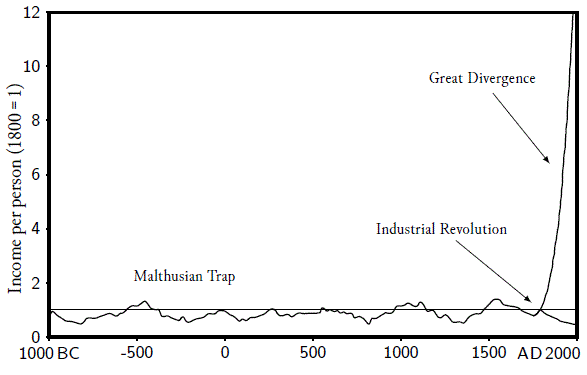
\includegraphics[width=1\linewidth]{img/ch1/fig2} \caption{Image from Gregory Clark, Farewell to Alms: A Brief Economic History of the World (Princeton, N.J.: Princeton University Press, 2007), p. 2.}\label{fig:fig102}
\end{figure}

One of the crucial national income accounting concepts is this thing called Gross Domestic Product, or GDP for short.

Definition: Gross domestic product refers to the value of final goods and services produced in a country within a particular period, usually a year.

A few remarks are in order:

\begin{enumerate}
\def\labelenumi{\arabic{enumi}.}
\item
  GDP is not an ``end all, be all'' measure of the quality of life. It is but one measure of the quality of life. It measures how much resources you have to buy stuff. It does not measure literacy, longevity, environmental quality and other measures of the quality of life we might care about.
\item
  When making comparisons of GDP across countries we need to make adjustments for country size. It will not be a surprise to anyone that the US has higher GDP than Norway. After all, the US has about 60 times as many people as Norway. So, when we adjust for population size by dividing each country's GDP by the number of people, we get for the year 2019.
  So, Norwegian GDP per person is about 15\% higher than in USA. That means that the average person in Norway has a purchasing power that is 15\% higher than the average person in the US.
\end{enumerate}

\begin{longtable}[]{@{}cc@{}}
\toprule
Country & Per Capita GDP (in USD) \\
\midrule
\endhead
United States & 65,000 \\
Norway & 75,000 \\
\bottomrule
\end{longtable}

\begin{enumerate}
\def\labelenumi{\arabic{enumi}.}
\item
  Sometimes when we adjust for country size, we divide GDP not by the population, but by the number of workers. When we divide by, or normalize, by population size we are asking the question: How much stuff is available for consumption per person. This is an opulence type question. When we divide by, or normalize by the number of workers, we are asking the question: How much stuff can each worker produce? This is productivity question. Both questions are certainly valid questions. What kind of data we collect will typically depend on the question we are after.
\item
  When making comparisons of GDP, total or per person, it is important that this is not done using the exchange rate of the two currencies used in the two countries. Exchange rates often fluctuate wildly from month to month, week to week, day to day, without really impacting the purchasing power for the typical residents of the countries. These comparisons must be made at what is called ``purchasing power parity'' to be meaningful.
\item
  When making comparisons of GDP, total or per capita, for one country over time, it is important to adjust for inflation. Inflation here means persistent changes in the price level. This is more important when comparisons are made over longer time spans rather than comparing GDP for two adjacent years, say comparing US GDP in 2020 to GDP in 1975. A gallon on gasoline at that time cost 57 cents.
\end{enumerate}

\hypertarget{basic-notation}{%
\section{Basic Notation}\label{basic-notation}}

Gross domestic product refers to production. Production requires inputs. In most economic models we will treat GDP as an output and we will assume for starters that there are two inputs, which we will call labor and capital. As a matter of notation, we will let

\begin{verbatim}
Y = GDP
N = the amount of labor used
K = the amount of capital used
\end{verbatim}

We can think of the amount of labor being measured either in the total number of workers employed or by the total number of hours worked by all workers in the economy. Capital is the collection of durable inputs used in production. Examples would be the robots on an assembly line, the trucks that bring lettuce from Imperial Valley to Indiana, the computers used for design, the shovels used in construction, etc.

In short we have inputs going in and GDP coming out. But how are the inputs transformed into output? We will refer to this as the production function, F. That is we can write the production function as

\[Y = F(K,N)\]

where F stands for any function which transforms our inputs to outputs. In most application the function F will have particular properties that are appropriate for the given application.

The production function at the level of an individual firm is an engineering description of the production process. There is very little, if any, economics here. If you are running a barbershop, you need barbers and scissors, to produce haircuts. If you are running an oil refinery you need chemical engineers and crude oil and a few other things to produce gasoline. To produce an iPhone you need rare earth minerals, cobalt and such. No cobalt, no iPhone.

At the level of an entire economy the production function is simply a relationship between the major inputs, things like capital and labor. Sometimes, (this depends on the application, the question at hand), we include raw materials, cobalt?, or energy.

A few things should be clear.

\begin{itemize}
\tightlist
\item
  If we use more capital, we will get more output. In ``math speak'' that is: The function F is increasing in K. That is when we hold the amount of labor constant.\\
\item
  The same is true for labor. Holding the amount of capital fixed, the more labor we employ, the more output we get. For a fixed level of K, the function F is increasing in N.
\end{itemize}

\hypertarget{measuring-economic-growth}{%
\section{Measuring economic growth:}\label{measuring-economic-growth}}

We let \(y_t\) denote real per capita GDP in period t. For all time periods t. Then \(y_{t+1}\) is GDP, real and per capita, for period t+1. We let gt denote the growth rate of real per capita GDP. Then we can define the growth of real per capita GDP from period t to period t+1 to be

\[g_t = \frac{y_{t+1} - y_t}{y_t}\]

We can calculate this growth rate for GDP for quarterly data, for annual data or at any frequency where data is available. What frequency we use depends on the particular question we have in mind. If we use quarterly or annual frequencies, we are most likely interested in business cycle questions. For questions of long run growth, we might take calculate growth rates over decades or even longer periods.

\hypertarget{a-thought-experiment}{%
\subsection{A thought experiment}\label{a-thought-experiment}}

This thought experiment goes back to Robert Lucas, Nobel Laureate of the University of Chicago\footnote{\url{https://en.wikipedia.org/wiki/Robert_Lucas_Jr}}. from the 1980s. This experiment shows the power of exponential growth.

\begin{longtable}[]{@{}
  >{\centering\arraybackslash}p{(\columnwidth - 6\tabcolsep) * \real{0.25}}
  >{\centering\arraybackslash}p{(\columnwidth - 6\tabcolsep) * \real{0.25}}
  >{\centering\arraybackslash}p{(\columnwidth - 6\tabcolsep) * \real{0.25}}
  >{\centering\arraybackslash}p{(\columnwidth - 6\tabcolsep) * \real{0.25}}@{}}
\toprule
Country & Annual growth rate & Doubling time & Income of grandchild/income of grandparent (in 1960-1985) \\
\midrule
\endhead
South Korea & 7\% & 10 years & 32 \\
India & 1.5 \% & 50 years & 2 \\
\bottomrule
\end{longtable}

This thought experiment is based on true data. The two numbers in the first column are the actual growth rates for these countries in that period. A South Korean grandchild will be richer than the grandparent by a factor of 32! This is assuming that a generation comes every 25 years, which is an eminently reasonable assumption. A factor of 32 is huge.

Remember this is per capita and it is already adjusted for inflation.\\
If we assume that India and South Korea had he same initial starting conditions in 1960, then after 50 years, the typical South Korean will be 16 times as well off as the typical person in India. That is a stunning difference in purchasing power.

To convince yourself of the enormous difference in the quality of life associated with such large growth rates of 7\% or so, google images of Seoul in 1955 and in 2015. What a difference, like night and day! (See Figure 3.)

Figure 3 What a difference economic growth can make

\hypertarget{the-rule-of-70}{%
\section{The Rule of 70!}\label{the-rule-of-70}}

The Rule of 70 is a convenient way to get an idea of how fast exponential growth can be. It allows us to calculate doubling times, if we know the growth rates.
- How long will it take for GDP to double if the average annual growth rates in x\%?
- How long will it take for my \$1,000 investment to double if the interest rate is y\%?
- How long will it take for Covid-19 infections to double if R0 , the average infection rate is 2.3?

The power of exponential growth is often underappreciated.

So here is the rule:

Doubling time = 70/g

where g is the growth rate.

Examples:

\begin{enumerate}
\def\labelenumi{\arabic{enumi}.}
\item
  If the growth rate is 3.5\%. then it will take 20 years for income to double.
\item
  The economy in China started to grow like gangbusters around 1990. After 1990 their growth rate has averaged about 7\% annually. At that rate incomes will double every 10 years. In 2020 Chinese per capita GDP was about \$10,000. Using the rule of 70 we can infer that Chinese GDP per person was:
  \$5,000 in 2010
  \$2,500 in 2000
  \$1,250 in 1990 (That is \$3.40 per day.)
\item
  In the US in 2020 GDP per capita is \$65,000. Over the past 120 years the US growth rate has averaged 1.8 \% annually. Under this growth rate it takes about 40 years for incomes to double. Then, if that continues, we can estimate future income levels in the US to be:
  \$130,000 in 2060
  \$260,000 in 2100
  Imagine that potential!!!
\item
  We can use the data from example 3 to go backwards in history. We can calculate incomes going back in steps of 40 years to get
  \$32,000 in 1980
  \$16,000 in 1940
  \$8,000 in 1900
  \$4,000 in 1860
  Of course, all these exercises work well if the growth rate remains constant at the indicated level. And we have to keep in mind that these are long run projections, approximations and that there can be deviations due to business cycles or other more short- term events\footnote{\url{https://en.wikipedia.org/wiki/Rule_of_72}}
\end{enumerate}

\hypertarget{the-solow-growth-model}{%
\section{The Solow Growth Model}\label{the-solow-growth-model}}

We will begin with a workhorse model that can provide some, but not all, answers. No model will ever provide all answers. In the model, named after Robert Solow, we will first trace out the evolution or growth of the capital stock.
\#\#\# Physical Capital Accumulation

Remember that the capital stock is a durable input in production, still like tractors, computers, warehouses, etc. As the input capital increases (declines) we can expect output, GDP, to increase (decline) accordingly. It will be convenient to follow the evolution of the capital stock. Once we figure out what happens with the capital, we can figure out what happens with GDP.

We will follow a small string of mathematical operations. The math may not always be clear to you. Simply return to the meaning of the variables. We try to show both the math and explain in words what the math means. To test your understanding you should be able to put the below equations into words as well.

We start with an accounting identity. \(K_t\) represents the capital stock today, \(K_{t+1}\) represents the capital stock tomorrow. We let \(D_t\) represent the amount of the capital stock that depreciates in that period and we let \(I_t\) represent the amount of new investments made in the period.

If this is a bit abstract think of a trucking company that owns 1000 trucks. That is their capital stock at the beginning of the year 2020. In that year, 20 trucks are retired and go to the truck graveyard. That would leave the company with 980 trucks. But the company buys 30 new trucks, so at the end of the year the company has 1010 trucks.

The other analogy we can use is water in a pond. During the day water evaporates and diminishes the amount of water in the lake. But at the same time, water enters the pond as well, through runoff from the nearby area and rain that may have ocurred that day.

We call depreciation and investment flow variables. They are like water flowing in and out of the pond. We call the amount of capital a stock variable. It is like the total amount of water in the pond.

Our first equation just says: The amount of capital tomorrow is the amount of capital today minus the amount that depreciates plus the amount that is invested. This is an identity.

\[K_{t+1}=K_t-D_t+I_t\]

This is the same thing as our pond example. Tomorrow's amount of water, will just be today's water, plus any that has flowed in, minus any that has evaporated.

To get to the second equation we make the assumption that depreciation is always a constant fraction of the total amount of capital. This is an assumption, that is not necessarily true. In some years there might be more accidents that destroy trucks than in others. There is a certain amount of randomness involved. Here we abstract from this randomness and assume constant depreciation. We call the fraction of the capital stock that depreciates \(\delta\). Of course, \(\delta\) is always between zero and one.

\[=K_t- \delta K_t+I_t\]

To get to the third equation we just use a bit of algebra. We recognize that the first two terms on the right side of the equation contain a common term \(K_t\). So, we factor it out to get the next line.

\[=(1-\delta) K_t+I_t\]

The next step is more substantial, much more substantial. Here we assume that all investment is financed by current domestic savings:

\[I_t=S_t\]

That is, the economy is closed. All investment in the domestic economy comes from domestic savings. The Japanese or the Chinese cannot invest on the US economy. We know that there is typically foreign investment in all economies. Here we rule this out. By assumption.

The first very basic national income accounting identity states:

\[c + i = y\]

where c is consumption, i is investment and y is GDP. This little identity says: Stuff is produced, and you can either eat it, c, or save and invest it, i.

All of this gets us to:

\[=(1-\delta)K_t+S_t\]

\(S_t\) is total savings in the economy in period t. Savings is that part of output that is not consumed.

We can then think that savings can be expressed as some fraction of GDP. That is if GDP is \$ 1,000 and savings was \$ 200, then savings in this case is \(0.2 \times GDP\)

Let's use s (lower case) to denote the savings rate in the economy. In the term \(sY_t\) we look at what is the fraction of total income in the economy that is actually saved. Then as we showed above, \(S_t=sY_t\).

\[K_{t+1}=(1-\delta) K_t+sY_t\]

As noted way back in our Basic Notation section, \(Y_t\) denotes output, or GDP in period t. That output is produced with inputs, capital \(K_t\) and labor input \(N_t\) according to the production function \(F\).

For our basic Solow Growth Model, we assume the production function has the following general properties:
- For a fixed amount of labor, the output is increasing in the amount of capital used, but at a decreasing rate.
- For a fixed amount of capital, the output is increasing in the amount of labor, but at a decreasing rate.
- In ``math speak'' the production function is assumed to be concave.
- In ``econ speak'', we say that the production function exhibits diminishing returns to each input.

So, we have in the equation below that output, GDP, is produced with two inputs, capital and labor, according to the production function F. The term \(A_t\) below denotes technological progress. (More on that later!)

\[=(1-δ) K_t+s[A_t F (K_t,N_t)]\]

In the next step we simply assume, for now, that the level of technology stats constant. The time subscript on A has disappeared. So, it does not change over time. This is an assumption that we are making, for now. We will address the question of technological progress later.

\[=(1-δ) K_t+s[A F (K_t,N_t)]\]

In the next step, we simply consider one specific example. In that example the parameter \(\alpha\) is any number strictly between zero and one. If \(\alpha\) is large, then capital is very important in production, relative to labor. If \(\alpha\) is small, then labor is more important in production. The appropriate value of \(\alpha\) will depend on the context. In poor countries, agriculture is very labor intensive, low \(\alpha\). In the US, agriculture is very capital intensive, high \(\alpha\).

The particular example below will allow is to illustrate all the important properties and predictions of the Solow growth model.

\[=(1-δ) K_t+s A K_t^\alpha N_t^{(1-\alpha)}\]

One more assumption: The population is assumed to be constant. So we can drop the subscript t in the above expression for \(N\).

In what we have done so far, we have let all variables be upper cases. Upper cases in this model will always denote totals. Upper case K denotes total capital stock, upper case Y denotes total output, upper case N denotes total employment.

We want to be able to express all or variables in per capita terms. Why?
- We want to be able to make statements about the income growth of the average or typical person and we want to get away from comparing apples, large countries like USA, China to oranges, small countries like Norway or Switzerland.
- We want to be able to compare average income of residents in any country, regardless of country size.

That is why we normalize everything from now by N, the size of the country and will express everything in per capita terms. We will let lower cases represent per capita terms. For example, \(k_t\) will be the per person/capita capital stock in period t. Similarly for the other variables.

Then, dividing both sides of the equation by N, the constant population we get
\[\frac{K_{t+1}}{N}=(1-\delta)\frac{K_t}{N}+sA(\frac{K_t}{N})^\alpha\]

Let \(k_t=\frac{K_t}{N_t} = \frac{K_t}{N}\) for all t.

Then we can write the above equation as:

\[k_{t+1}=(1-\delta) k_t+s A k_t^α\]

This is the ultimate expression we will be working with. In our model, this equation will encapsulate the entire evolution of the capital stock. And we can calculate the entire sequence of capital stocks from any arbitrary initial starting point for as long as we like. For the US potential starting points might be the years 1565, 1620 or 1776. For Germany two potential starting points could be 1945 or 1990.

How does this work? Suppose we have estimates for the parameters \(\alpha\), \(\delta\), \(s\), and \(A\). If we also have an estimate for the initial capital stock \(k_0\), say for the US in the year 1776, then we can plug all these estimates into the above equation and calculate \(k_1\), the per person capital stock in period 1. Then we take \(k_1\), the value we just calculated and feed it into the equation to calculate \(k_2\). The we insert \(k_2\) into the equation to calculate \(k_3\).
Etc.
Etc.
Etc.
Until the cows come home.

If you are good with spreadsheets or coding, you can try this. Just pick some values for the above parameters and see what happens, how the capital stock grows over time.

There is an alternative way to see how all of this works. Consider Figure \ref{fig:fig104} below. That figure contains the graph of the above equation with kt on the horizontal axis and \(k_{t+1}\) on the vertical axis.
The graph is concave. It must be concave since one part, the first part, is a straight line with slope \((1 - \delta)\) and the other part \(sA(k_t)^\alpha\) is a concave function. So, the sum of the two is also a concave function. This concave function is the one graphed below.

\begin{figure}
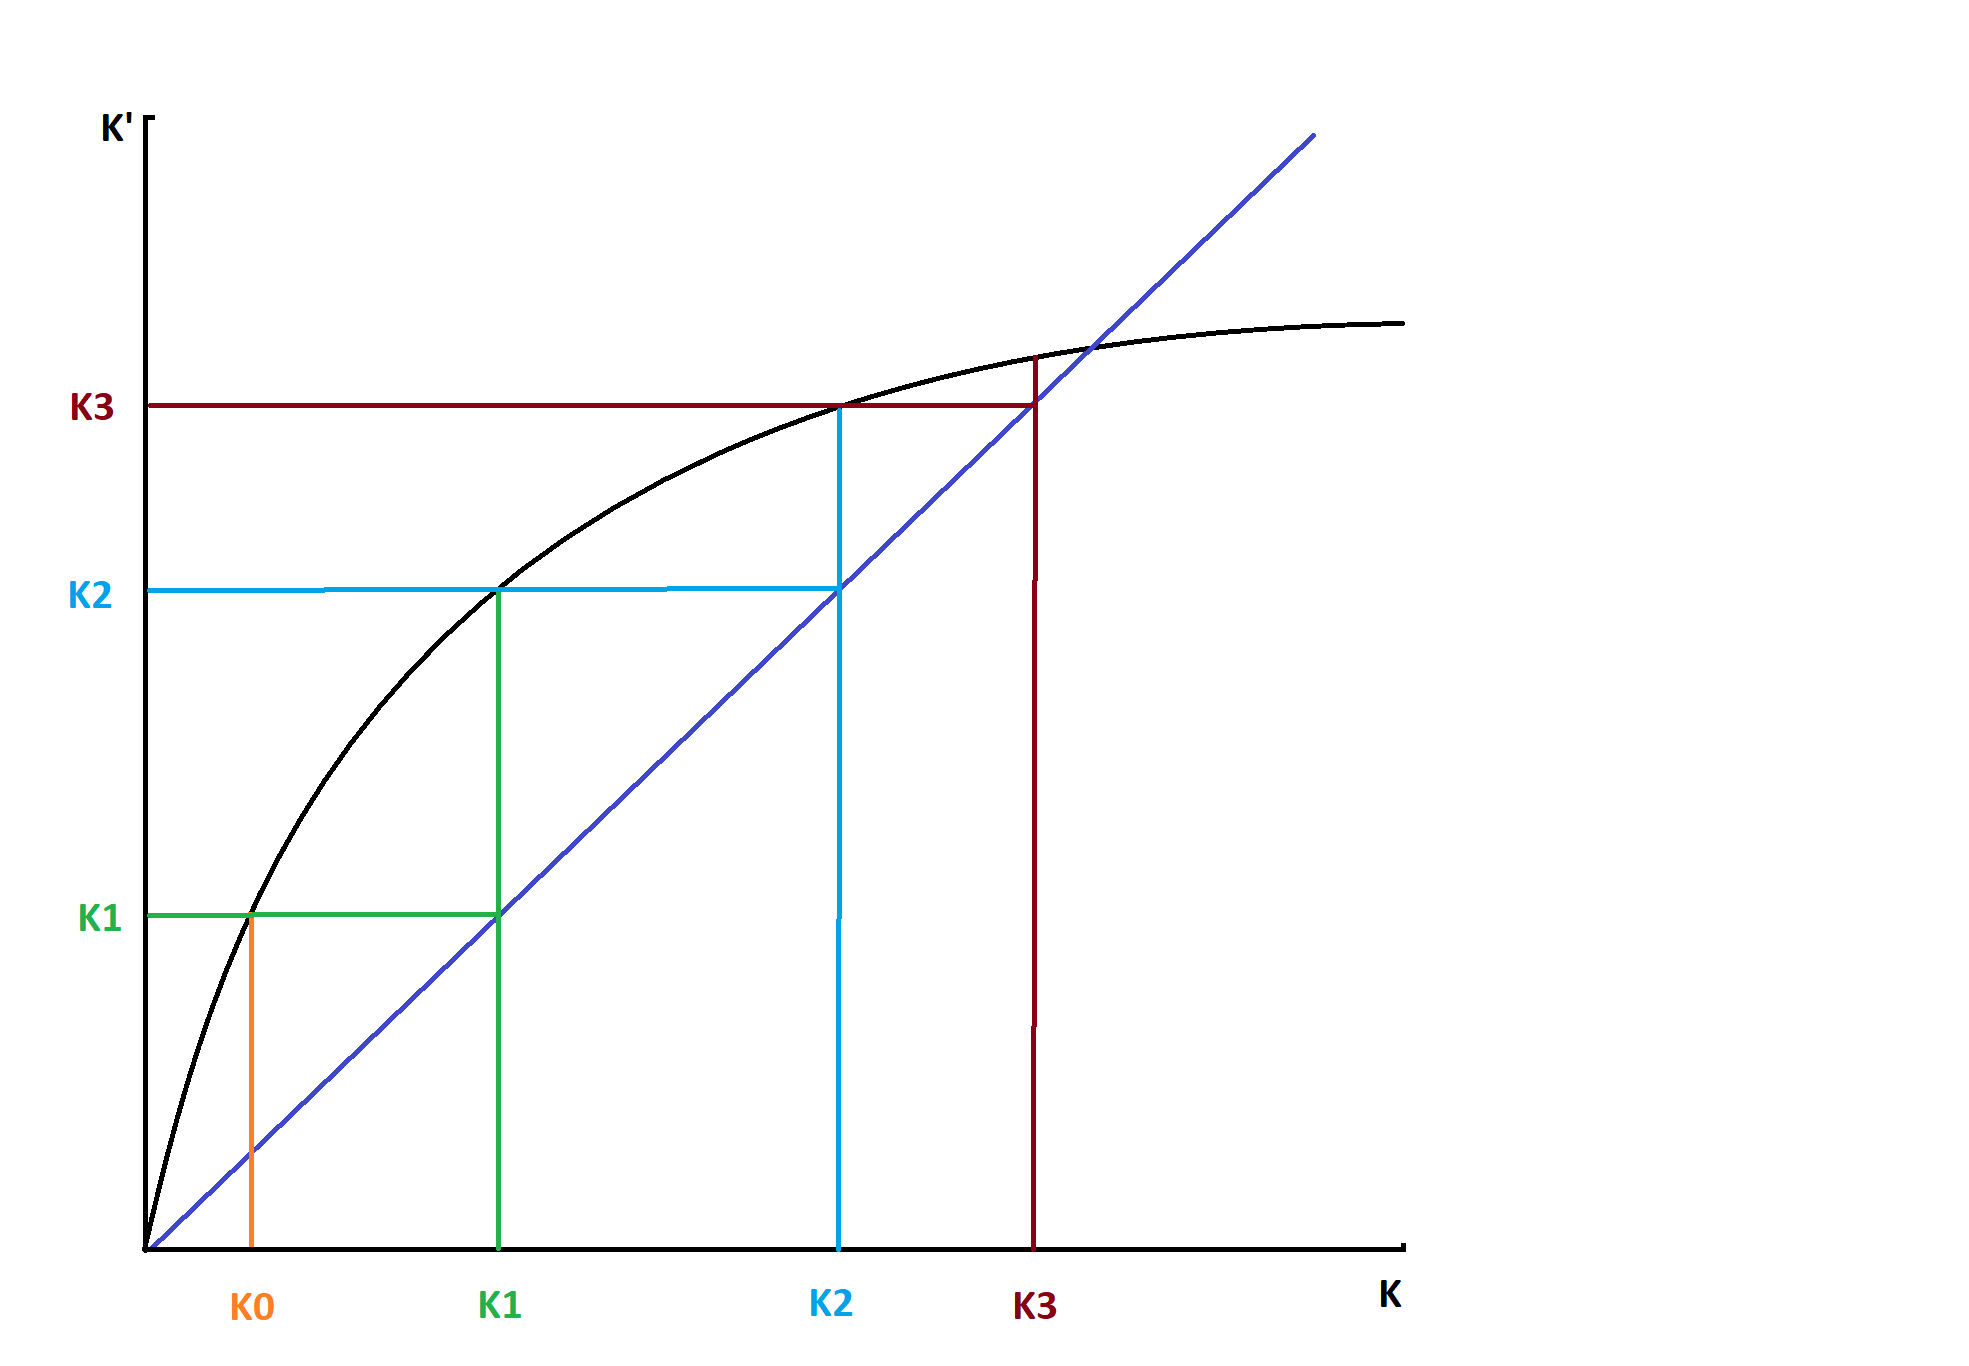
\includegraphics[width=1\linewidth]{img/ch1/k3} \caption{Illustration of Capital Stock Evolution in Solow Growth Model.}\label{fig:fig4}
\end{figure}

We start with \(k_0\) and calculate \(k_1\). We do this by starting at \(k_0\) on the horizontal axis and from there we go up vertically to the graph and then read off \(k_1\) on the vertical axis.

Then we take that value of \(k_1\) on the vertical axis, go over to the 45-degree line and from there go down to the horizontal axis. Now we have \(k_1\) on the horizontal axis. This works because the 45-degree line has a slope of one, which means that the rise is exactly the same as the run. From the origin up to \(k_1\) that is the rise. From the origin over to \(k_1\) that is the run.

We repeat this process: From \(k_1\) go up to the graph, then over to the vertical axis to read of \(k_2\). Bring that value of \(k_2\) from the vertical axis over to the 45-degree line, then go down to the horizontal axis and mark that value of \(k_2\) there.
Repeat.
Etc.
Etc.

\href{https://i.imgur.com/IZTZUav.gif}{This animated graphic along with the text above may help understanding in what is going on.}

If we look carefully at the graph above, we see

Prediction 1: The capital stock in an economy increases over time at a decreasing rate. Eventually the capital stock reaches the steady state level ks.

For any economic variable, the steady state value is that one that stays constant forever once it is reached.
In the graph above we see that the capital stock increases and gets closer and closer to the value ks. Once the capital stock approaches the value where the graph crosses the 45-degree line, there is no escaping. Once you reach that value, you stay there. Forever. That is the steady state level of the capital stock.

Prediction 2: GDP in an economy increases over time at a decreasing rate. Eventually, the GDP reaches a steady state level.

This prediction follows directly from prediction 1. There are two inputs in production, labor and capital. Labor is fixed by assumption. Capital increases over time. Therefore, output, GDP increases over time. And if capital increases at a decreasing rate, then output must, by necessity, increase at a decreasing rate as well. And if capital reaches a steady state, then GDP must reach a steady state as well.

One of the obvious consequences of the second prediction is that eventually output, GDP, will stop growing. There will be no more growth. That is, essentially, just another way of saying that GDP reaches a steady state level.\\
The reason is simple: Since there are diminishing returns to capital, at a constant savings rate, over time, less and less will be invested in new capital. As less and less gets invested, the capital stock grows less and less and as a consequence, GDP grows less and less. Eventually, the growth of capital and of output has to come to an end.
Prediction 2': Consider two economies that are equal in all aspects, they have the same parameter values, but they differ in their initial level of capital per person. Then the growth rate of the economy with lower initial capital stock will have higher growth rates and therefore catch up with the richer economy.
This is known as The Convergence Hypothesis: GDP per capita in these economies is predicted to converge. Whether this is true in the data, in which data and to what extent is an interesting question and there is a large literature on this issue.

\hypertarget{solow-model-and-data}{%
\section{Solow Model and Data}\label{solow-model-and-data}}

We will start with data on three large economies, The United States, Japan and China going back to 1950s. We will be utilizing \href{https://www.rug.nl/ggdc/productivity/pwt/?lang=en}{Penn World Tables} for the data. In the supplemental materials we include the code used to generate the figures.

Comparing the US to Japan between 1960 and 1990 we see what looks like convergence. The difference between the two incomes is getting smaller in that time period. Those of us who followed the news in the 1970s and 80s recall a sense and perhaps a fear that Japan would overcome to US and become the dominant economy in the world. In hindsight this fear was totally unfounded. Even in the 1980s, Japanese income was still much, much lower than US income.

\begin{figure}
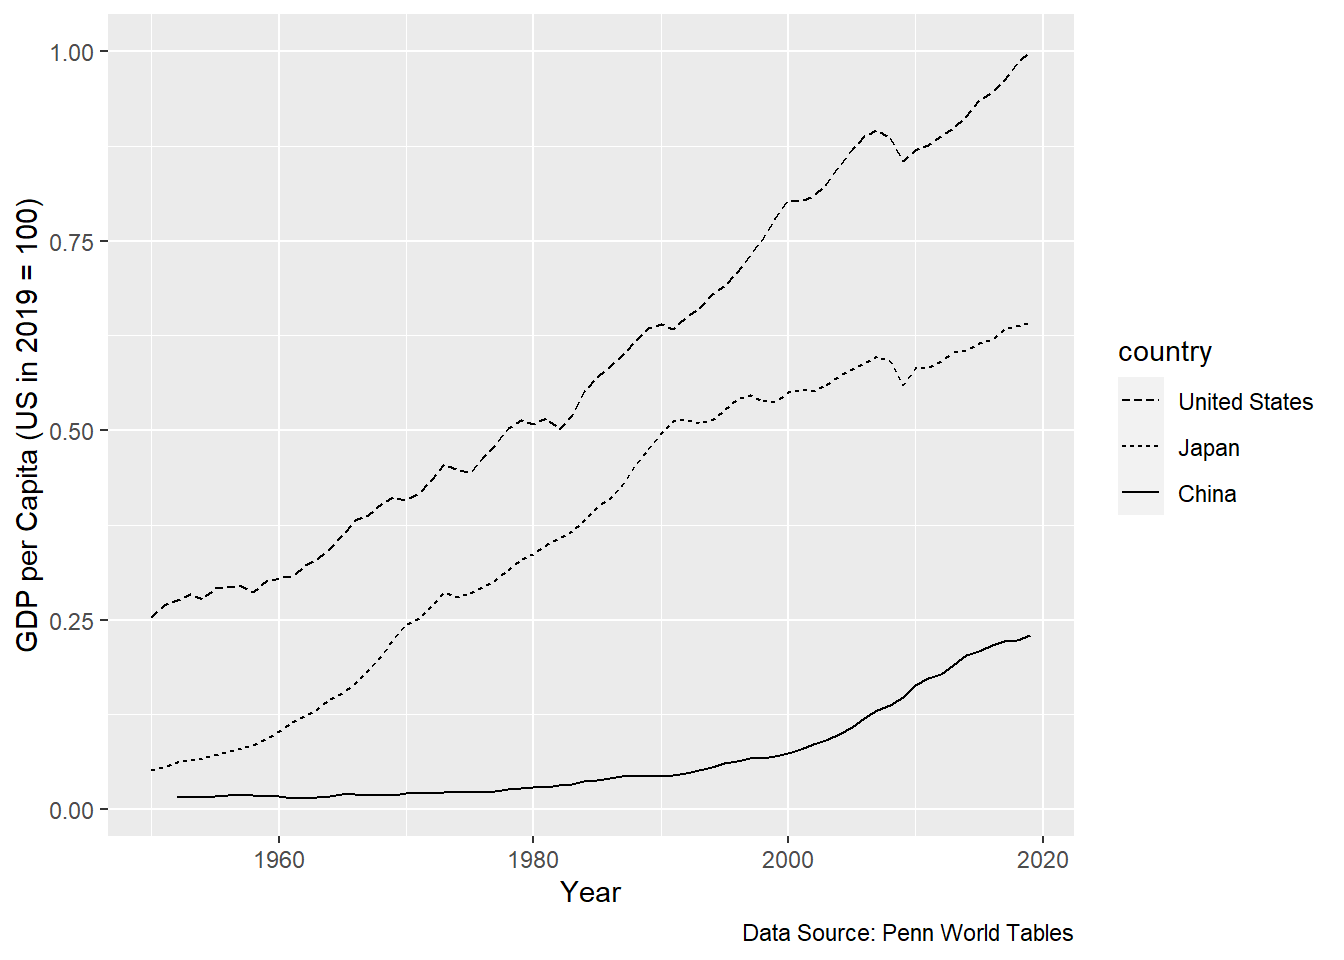
\includegraphics[width=1\linewidth]{bookdown-demo_files/figure-latex/fig105-1} \end{figure}

And then something happened in Japan. Growth went AWOL. It disappeared. The US economy kept on growing. The gulf between these two economies widened.

The punchline: Solow like convergence between the US and Japan? Yes, but only initially. After 1990, definitely divergence.

How about the China-US comparison? That comparison only makes sense after 1985 or so. The period before 1980 was plagued by very destructive periods and initiatives such as the Cultural Revolution. It is not surprising that incomes cannot grow under such circumstances. But after 1990, there is a definite convergence between US and Chinese average income. The Chinese economy seems to have grown at unprecedented rates for a long time. There is now, if you follow the news, a fear that the Chinese economy will catch up with the US economy and even overtake it.\\
But: what the future will bring remains to be seen.

The next figure below, Figure \ref{fig:fig106}, illustrates similar stories, not in terms of levels of income, but in terms of growth rates. The growth rates are 10-year averages so as to filter out business cycle changes. We want to filter out, ignore, the business cycle stuff so we can focus on long run growth.

\begin{figure}
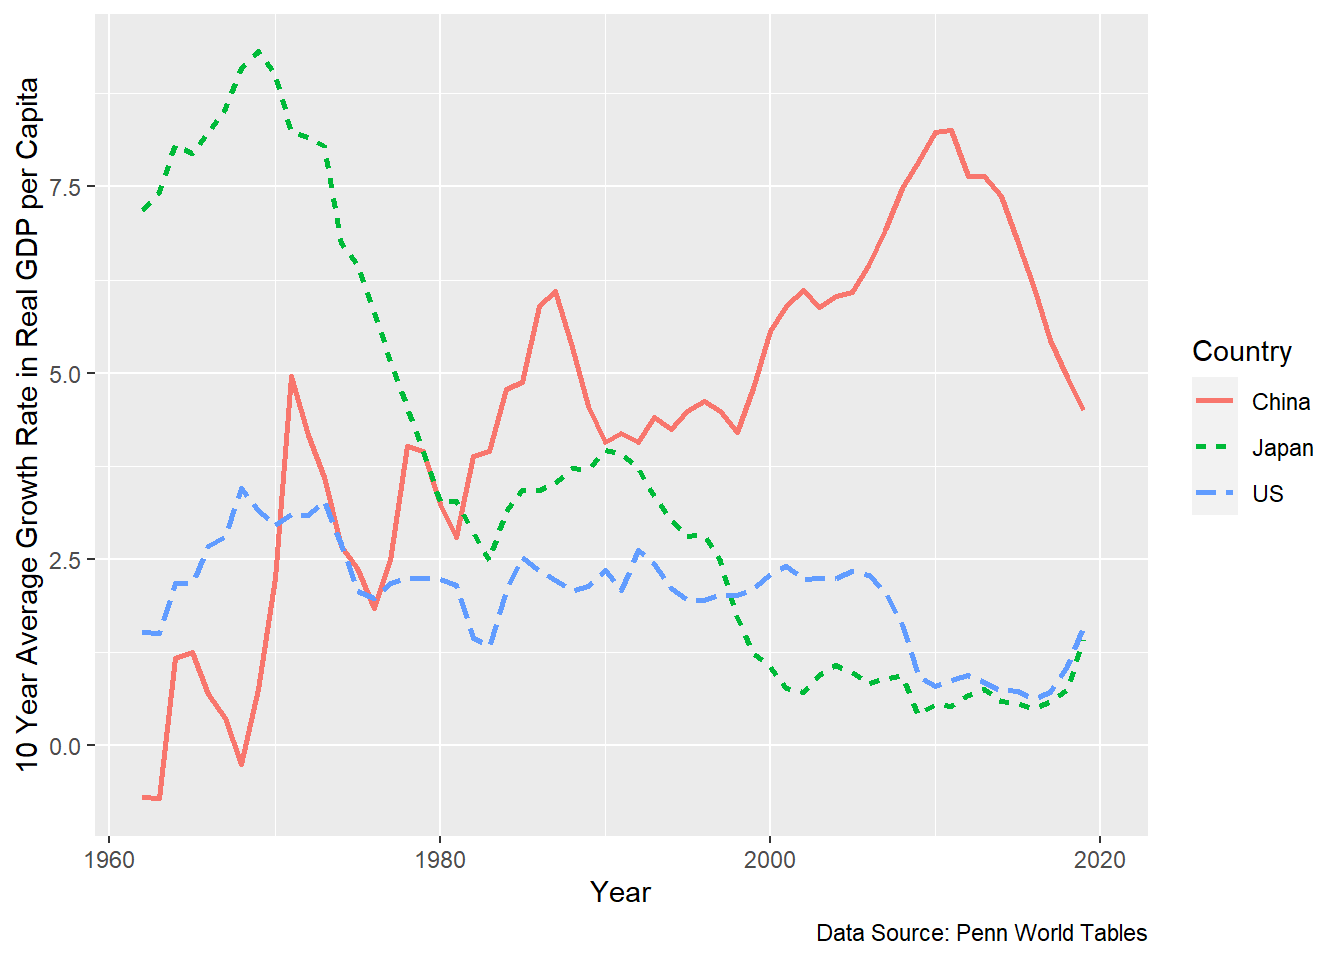
\includegraphics[width=1\linewidth]{bookdown-demo_files/figure-latex/fig106-1} \caption{High growth rates in poor countries, low growth rates in rich countries.}\label{fig:fig106}
\end{figure}

For the US the growth rate looks rather constant. There are some ups and downs, but if we tried to fit a straight line into the US observations, that straight line would be rather flat without any clear trend. That is not exactly good news for the Solow model. The Solow model predicts declining growth rates. It is hard to see declining growth rates in these data for the US.

The data on Japanese growth rates look more like the Solow prediction. Even though there are wild swings in these growth rate data, the overall trend is clearly downward. Of course, it is a fair and useful question to ask why there was such a large upward spike in the Japanese growth rate in the 1990s, or, perhaps equivalently, such a huge drop in growth rates in the 1970s and 80s. But here we are concentrating on more long-term phenomena. For Japan, the overall trend in the growth rates is clearly down, which is consistent with the Solow model.

How about China? The growth rates for China are rising, inexorably basically starting from the 1960. This seems to be in total contradiction to the Solow model. True. But I think we need to remember that in the 1970s China is emerging out of the Maoist economy with all its shortcomings and distortions. The Solow model was not designed to answer any questions about such transitions. It was designed to answer questions about stable market economies like the US or France or Norway or Japan. So, the failure if the Solow model to be consistent with the data is not really a failure of the model.

The failure of your TV to take you to the Chicago airport is not a failure either. It was not designed to do that.

\hypertarget{post-wwii}{%
\subsection{Post WWII}\label{post-wwii}}

The Solow model does well in the post WWII context. See the Figure below. In 1945 Germany, France, the UK were all more all less bombed out. See the picture of Dresden in 1945 below in Figure 7.

Figure 7 Not much capital there.

Without a doubt, the US at the time was the biggest economic power with the highest per capita income. Figure \ref{fig:fig108} below shows: (i) initially the growth rates were high and then they declined over time. (ii) the growth rates in the bombed-out countries were higher than in the US. In Europe, we see large scale conference of real per capita incomes. This convergence is certainly consistent with the Solow model predictions.

\begin{figure}
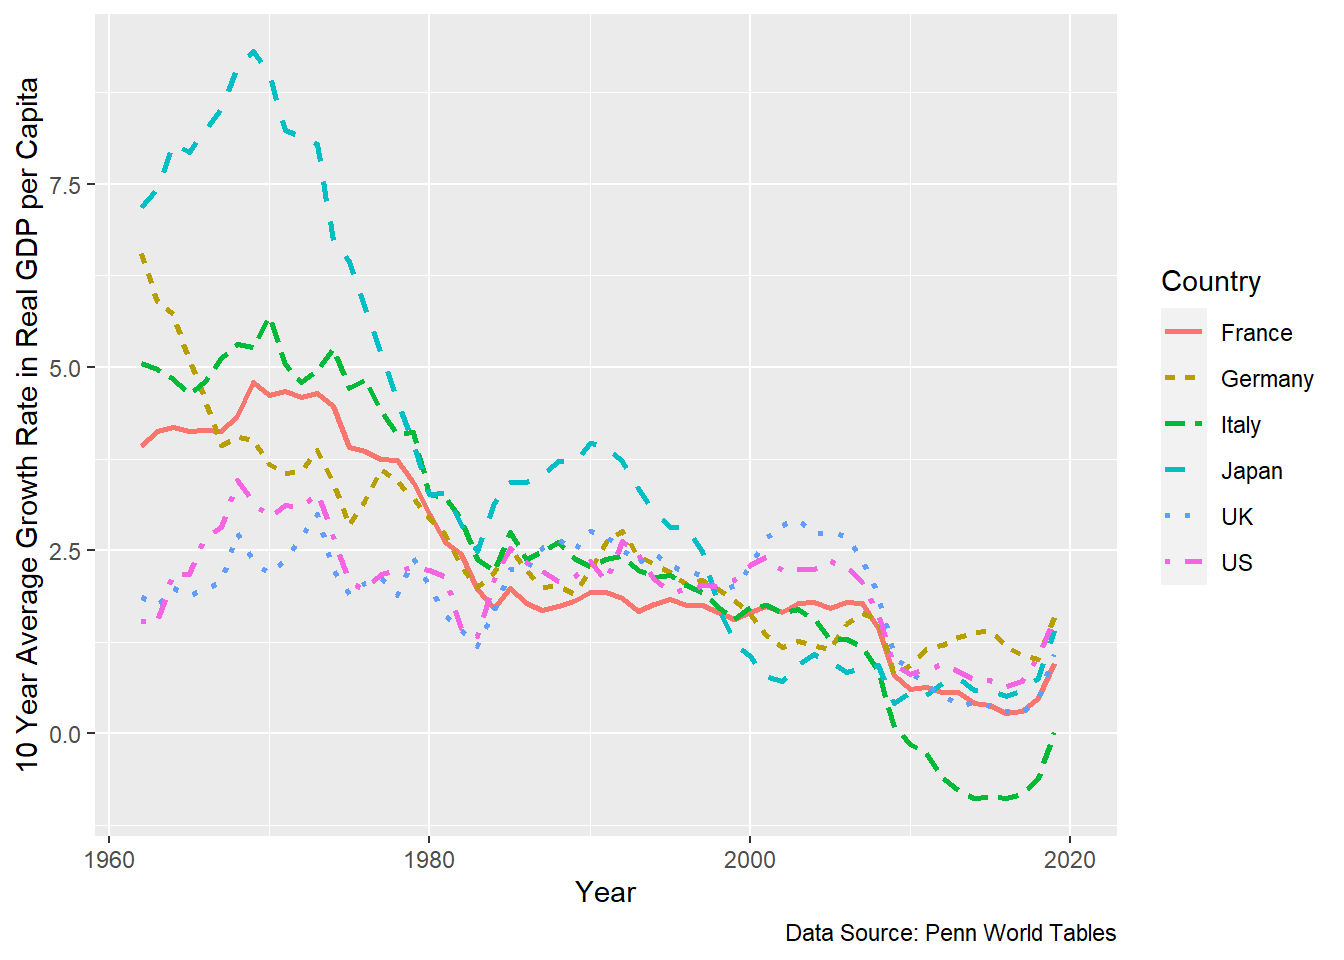
\includegraphics[width=1\linewidth]{bookdown-demo_files/figure-latex/fig108-1} \caption{High growth rates in poor countries, low growth rates in rich countries.}\label{fig:fig108}
\end{figure}

If we take a larger sample of countries in Figure \ref{fig:fig109}, we see some evidence of convergence. See below. Countries with higher(lower) levels of income experience lower(higher) growth rates.

\begin{figure}
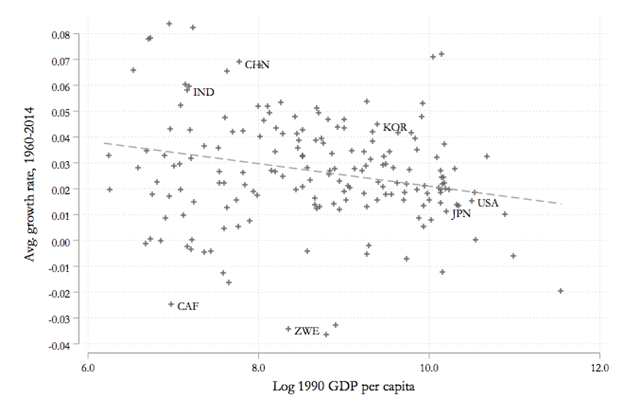
\includegraphics[width=1\linewidth]{img/ch1/growth9} \caption{High growth rates in poor countries, low growth rates in rich countries.}\label{fig:fig109}
\end{figure}

This is for relatively short periods. But if we take a longer historical view, going back 250 years with a larger set of countries, as in Figure \ref{fig:fig110}, we see not just divergence, but DIVERGENCE BIG TIME. This is actually the title of the paper from which the picture below is taken.

\begin{figure}
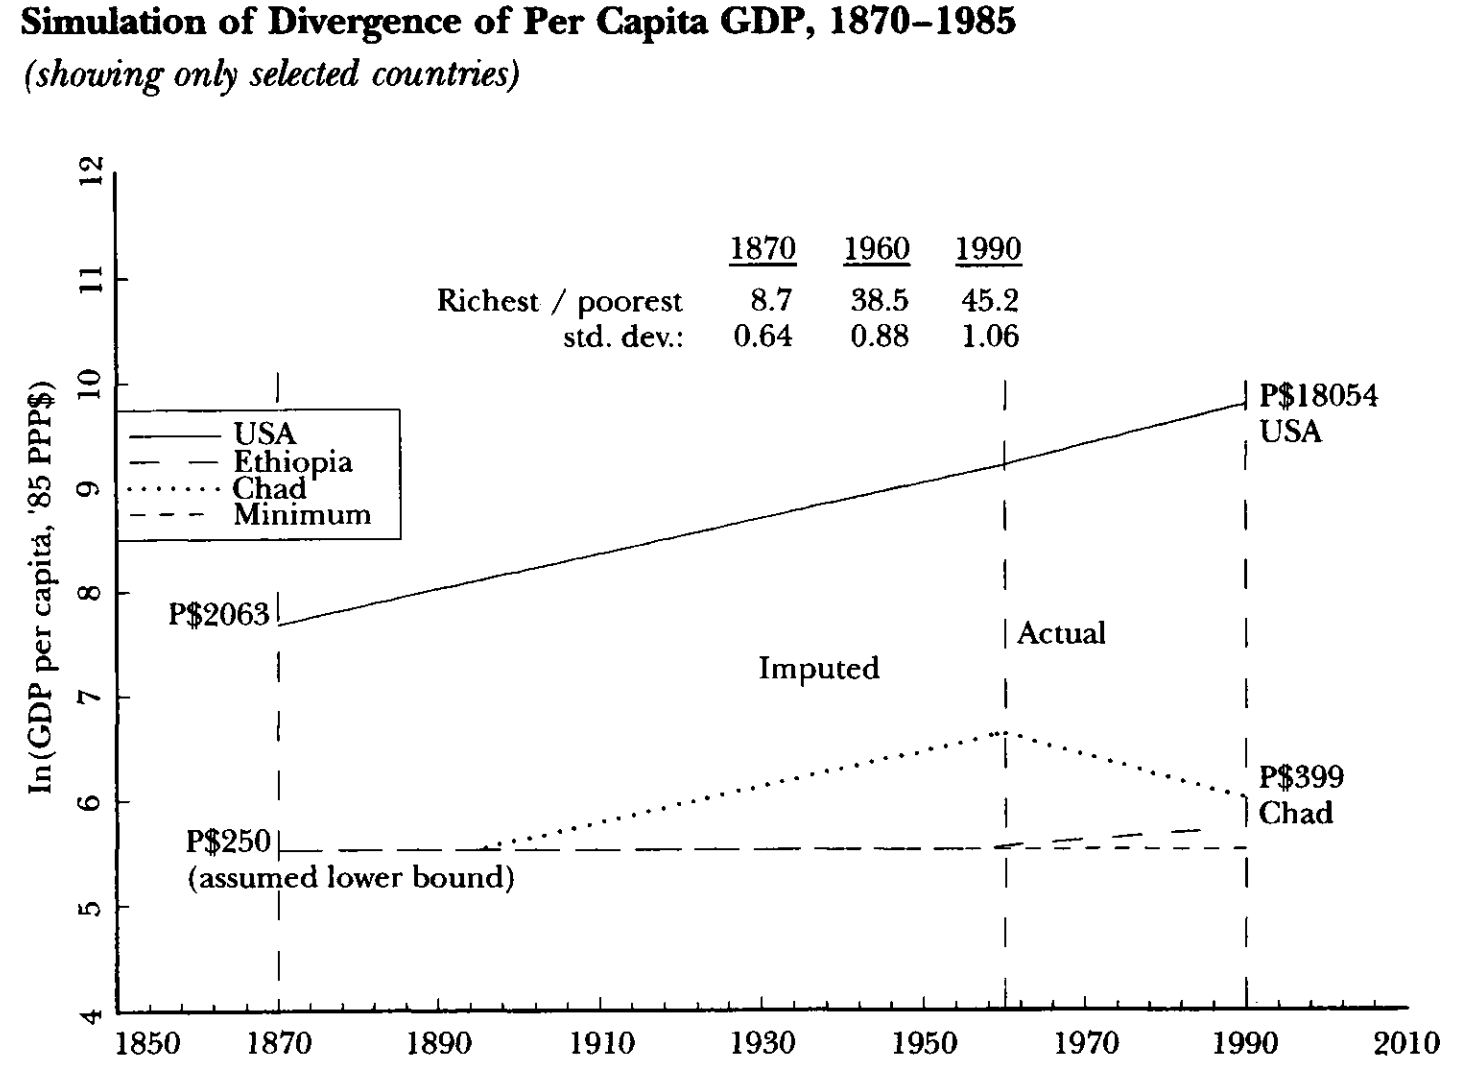
\includegraphics[width=1\linewidth]{img/ch1/growth10} \caption{Massive divergence over the long haul. Source: Pritchett, Divergence Big Time, 1997.}\label{fig:fig110}
\end{figure}

The data in the next two figures, Figure \ref{fig:fig111} and Figure \ref{fig:fig112}, for the US are also not kind to the Solow model. These figures contain data about long run growth in the United States. The figure below shoes the data for real per capita income for the US from 1880 to 1987. The vertical axis is on a logarithmic scale. Using the logarithmic scale makes it easier to see whether growth is constant, increasing or decreasing over time. If you look at the picture you see something that is truly amazing: an almost perfect straight line, with the obvious deviation of the Great Depression and WWII. Apart from that: A perfect straight line.

Absolute constant growth. Over a very long period.

You can even use the data from before the Great Depression, fit a straight line into that subset of the data and use that straight line, the data from before the Great Depression, to ``forecast'' income, real and per capita in 1985. If you did that you would be off by the price of a decent hamburger. In other words: that forecast is right on the money.

This exercise was actually performed by Charles Jones, in the paper mentioned below.

The punchline: In that 100-year time period, the growth rate in the US of real per capita income is constant.

That is a blow to the Solow model.

\begin{figure}
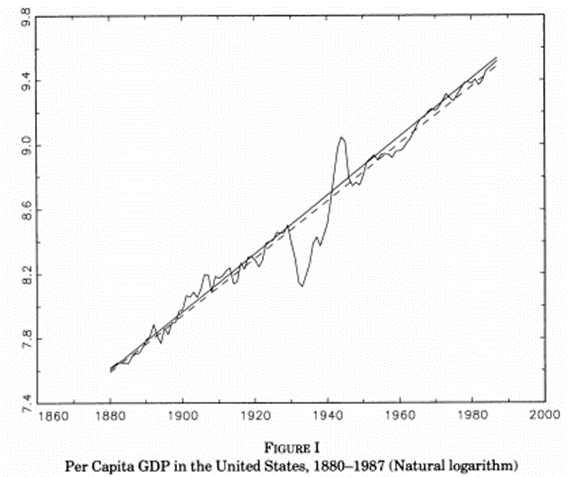
\includegraphics[width=1\linewidth]{img/ch1/growth11} \caption{On a logarithmic scale growth for US looks very constant. Source: Jones, Charles, Time Series Tests of Endogenous Growth Models, QJE 1995.}\label{fig:fig111}
\end{figure}

The next graph makes the same point of constant growth in a different way and points out why the constant growth is really very remarkable.
The bottom panel shows the growth rates of real per capita GDP for the US economy again roughly for a 100-year period. Of course, there are fluctuations, ups and downs. But, if you fit a straight line in the data, it is flat. Totally flat.

The growth rate is constant in this period.

At 1.8\% annually.

This is a number you must remember.

Why is this number important? In just about every election going back to the 1980s, some candidate for President promises to pursue a policy or set of policies that will increase the growth rate to 4\% or higher.
Is this reasonable? Believable?

When these candidates promise 4\% growth or higher, they usually do not talk about per capita growth, so we have to think about that a bit carefully. Over the last 50 years the population growth rate has been less than 1\% per year with a clear downward trend.

If we add the 1.8\% of real per capita growth and at most 1\% of population growth we get 2.8\%. And that is an optimistic upper bound since population growth has been declining. So, any politician who promises 4\% or higher must have something up his/her sleeve that is not revealed in the historical record. Perhaps these candidates know something that we don't know. But then it would be incumbent on them to fill us in on all the details of how such high growth can be accomplished. Otherwise, why would/should we take such claims seriously?

The figure below also points to why the constancy of the growth rate is really an amazing thing. The top panel shows the fraction of GDP collected as income taxes. This fraction increases massively in that period, yet there is no discernible influence of this huge tax increase on the growth rate. Perhaps that is amazing. But there is more.

Over this period education has also increased massively. More and more students are going to college. Average or median years of schooling have increased, almost doubled. This has no discernible impact on the growth rate.

The fraction of women entering the labor force has increased massively over this period. Female labor force participation increased from about 32\% in 1950 to about 60 \% by the year 2000. Again, there seems to be no discernible impact on the growth rate.

Longevity has increased tremendously. Life expectancy has increase from about 46 years in 1900 (that is for males) to about 74 years one hundred years later. This huge increase in life expectancy does not seem to have made any difference to the growth rate.

None of these changes seems to have had much, if any, impact on the economic growth rate. Perhaps that does qualify as being totally remarkable.

\begin{figure}
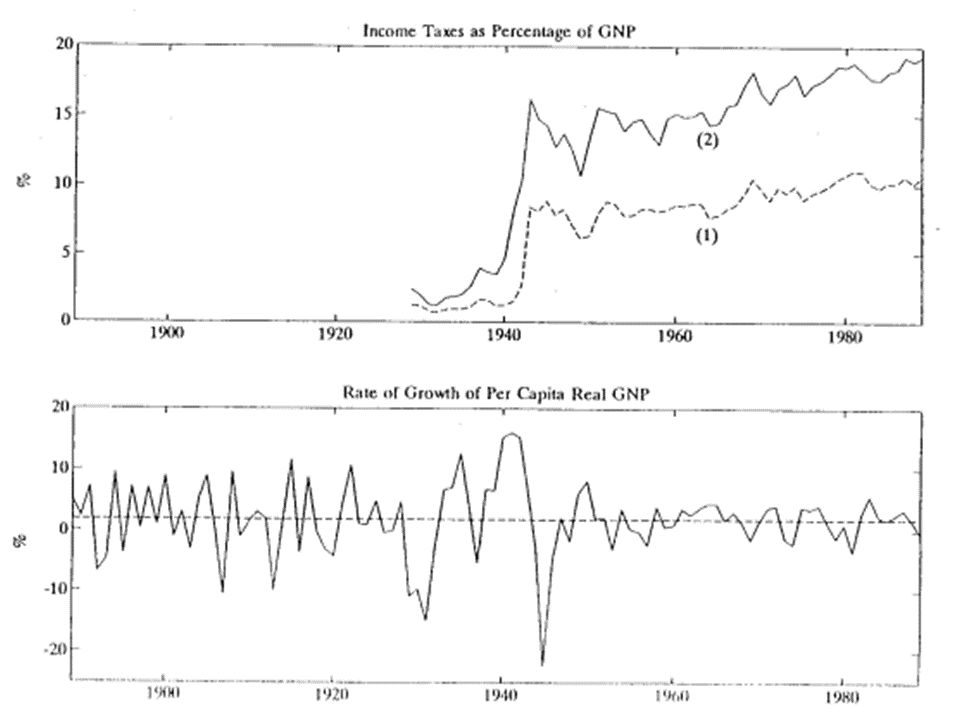
\includegraphics[width=1\linewidth]{img/ch1/growth12} \caption{Constant growth rates. Source: Stokey, N. and S. Rebelo, Growth Effects of Flat Rate Taxes. JPE, 1995.}\label{fig:fig112}
\end{figure}

If we take data for more recent years for the US, we see, In Figure \ref{fig:fig113}, evidence of declining growth.

\begin{figure}
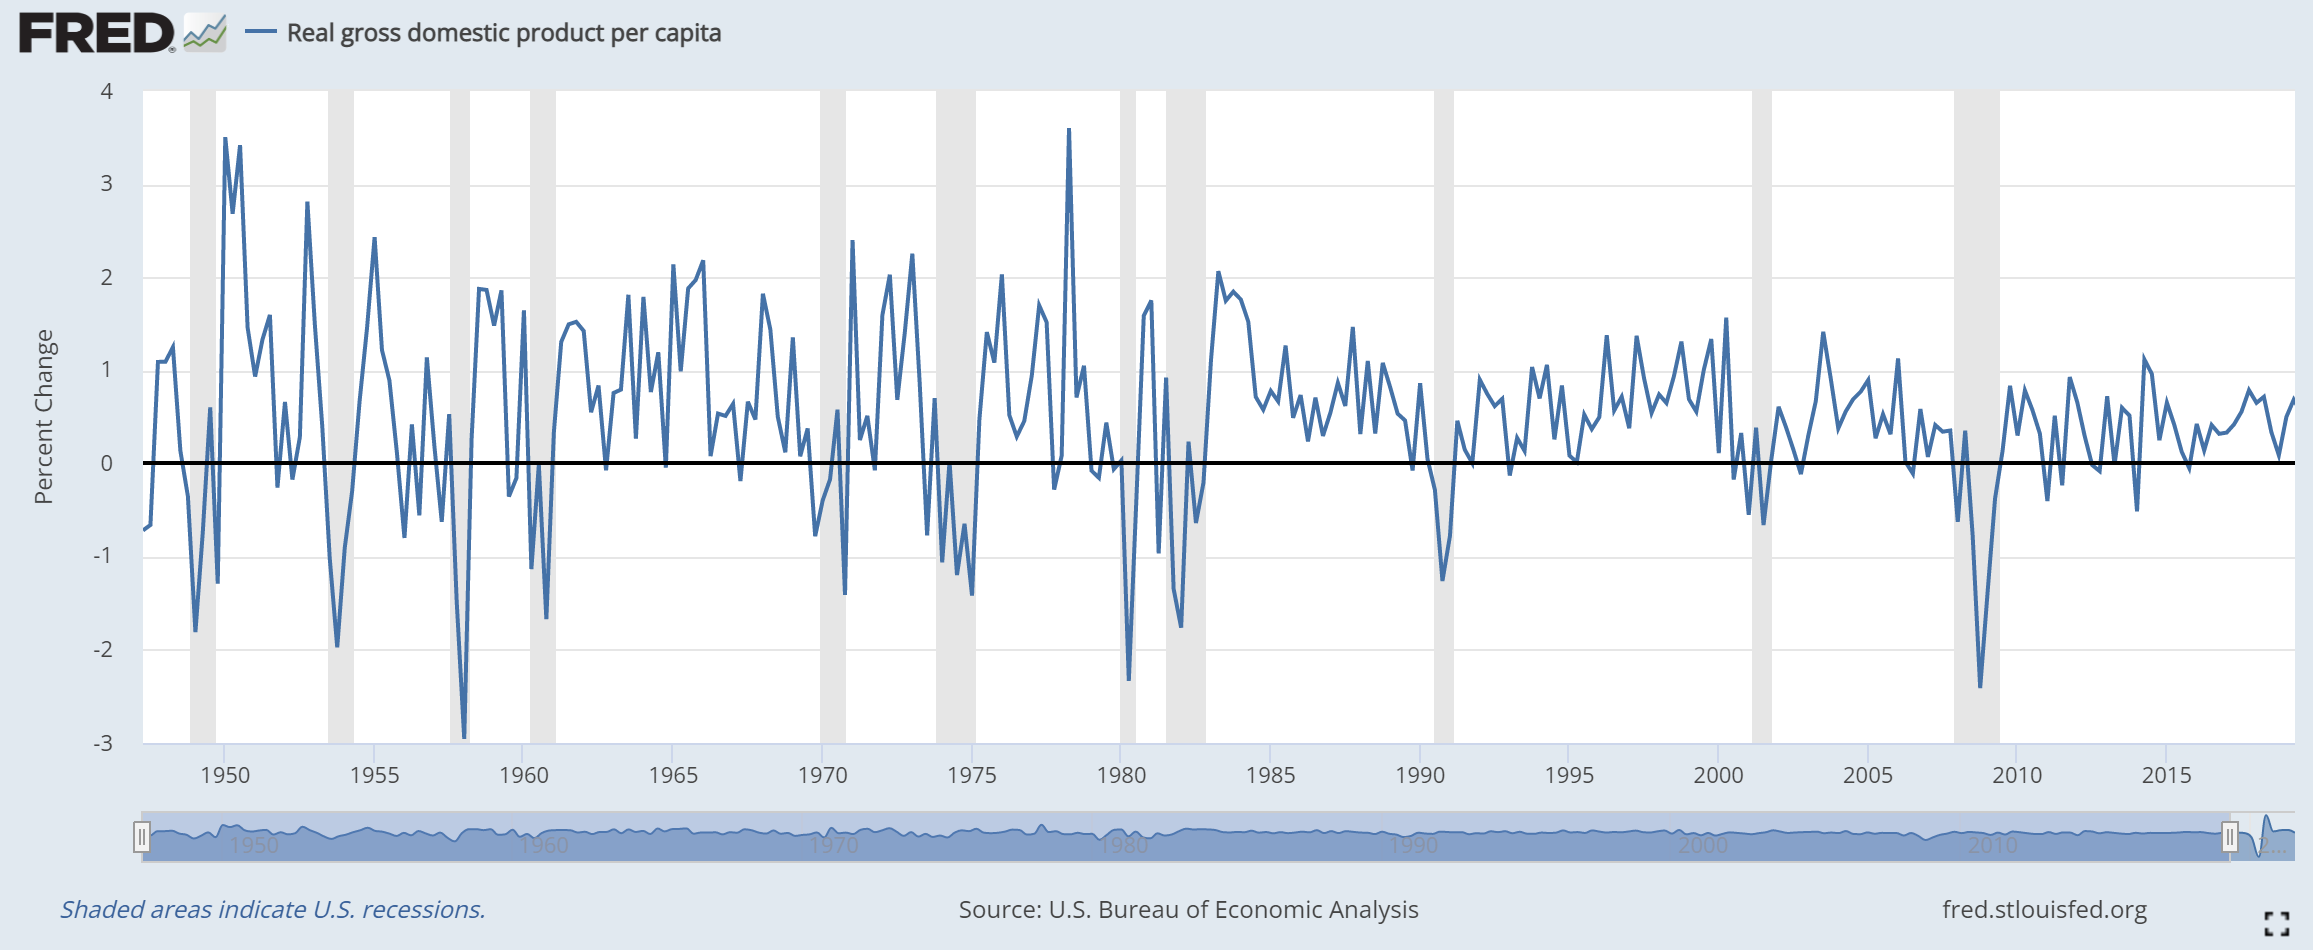
\includegraphics[width=1\linewidth]{img/ch1/growth13} \caption{Evidence of declining growth rates. Source: FRED}\label{fig:fig13}
\end{figure}

We will have to confront the questions:
- Why have growth rates in the US been declining?
- Is this decline good or bad?
\#\# Human capital accumulation

In the Solow model we considered in the previous sections, there was only one factor to be accumulated: physical capital. In this section we will allow for two augmentable factors: physical capital and human capital.\\
By human capital we simply mean all the marketable skill. In the Solow model the production function is given by
\[y_t=A F(k_t)\]

Recall that when we hold labor constant, then output is basically a function of capital only and the production function exhibits diminishing returns to capital.
We will now generalize the production function to

\[Y_t = A F (K_t, H_tN_t)\]

In this formulation \(N_t\) stands for labor as before. Labor could be measured by the total number of people employed or by the total number of hours worked. \(K_t\) is the total capital stock, \(Y_t\) is output of GDP and \(A\), as before is a measure of technology.

What is new here is \(H_t\), which stands for human capital. What we do here is we multiply \(H_t\) and \(N_t\) together to get

\[H_tN_t\]

We call this product ``effective labor''. We can think of \(N_t\) as hours worked. If we multiply the hours worked \(N_t\) with skill or human capital \(H_t\) we can get a measure of how much can be done or accomplished in the time spent working. We will refer to \(N_t\) as ``raw labor'' and to \(H_tN_t\) as ``effective labor''.

Effective labor varies both across countries and over time. The average Norwegian worker has more human capital and thus more effective labor then the average Nepali worker. Also, the typical American worker now has more human capital than the typical American worker had 100 years ago.

Just like physical capital, human capital can be accumulated; it can grow. It can also depreciate or become obsolete.

There are multiple ways to accumulate human capital.

\begin{itemize}
\tightlist
\item
  Formal schooling
\item
  Learning on the job
\item
  Leaning by doing
\end{itemize}

There is a large literature on each one of these components. Here we will focus on formal schooling, partially because in many countries formal schooling budgets take up large fractions of national income, GDP. In some cases, this is more than 5 or 6 \% of GDP.

So, one way to measure formal schooling is through expenditures. How much do we spend as a fraction of GDP on formal public education? When answering this question we have to be cognizant of the fact that there is also a significant private expenditure in formal schooling.

The second way to measure formal schooling or education is simply to ask how much schooling, how many years of schooling do students get. Of course, in every country there will be a distribution. Often, we categorize this the different stages of education completed, such as college completion or high school completion.

Figure 14 below shows that education in the US has increased tremendously. The fraction of the labor force that has completed college has increased substantially while the fraction of the labor force that has only finished elementary education or not finished high school has fallen drastically.

GENERATE THIS IMAGE
Figure 14 Increasing schooling time

Most countries have seen similarly large increases in years of schooling. Measured in average or median years or schooling. Or measured in the fraction of the labor force that has completed college.

Beware of measurements!

Measurements should be useful for the purpose at hand.

Measurements should not be too costly.

Both of these are worthwhile considerations.

But, sometimes measurements are taken simply because they are cheap. Please consider the link below. There are reports from central planning in the Soviet Union by plans being fulfilled by a very small number of huge nails or, alternatively, by a huge number of tiny nails. It all depended on the specifications given by the planner to the factory.

See the cartoon below.

\url{https://www.quora.com/Whats-the-meaning-of-this-Soviet-cartoon}

Incentives work!

They work really well.

There is a similar story about shoes in the Soviet Union. People were always lining up for shoes. Always. I mean always. It turns out that the Soviet Union at the time produced hundreds of millions of shoes per year. More shoes than were produced in the US.

The problem: They were just shoes, but not shoes consumers wanted. They were just not comfortable. And forget fashionable.

So the statement above about people standing in line for shoes needs a qualification. People were standing in line not just for shoes, not just for any pair of shoes. They were standing in line for comfortable shoes, for durable shoes, for practical shoes, for shoes that fit their needs.

Why am I telling you nail and shoe stories?

In education there is the risk, that we are looking at numbers, data, measurement in a way that is very similar to the way data were looked at in the nail and shoe stories.

In education we sometimes look at numbers that are easy to collect. And sometimes these numbers are not meaningful. Or at least, it is not clear how meaningful they are.

\begin{itemize}
\tightlist
\item
  Years of schooling.
\item
  The fraction of 18 years olds going to college.
\item
  The number of hours spent studying
  All these data fall into the category of questionable data. Whether data is questionable ALWAYS depends on a particular purpose: Is that data useful for my particular purpose?
\end{itemize}

So what could/would be our purpose here? We would hope that education makes people more productive. If education makes people more productive, we would see the effect of education in GDP.

Now, before we take a closer look at the connection between education, we can use some introspection to think about how useful or how accurate the above three measure can be.

Go back to high school and think of all the students who were you in graduating class. At that point they all had 12 years of schooling. Now consider the difference, if there is any, in the marketable skills among all the graduates in your class? Is that difference small? Is it large? How much do we miss in terms of productivity if for all these students, we just record 12 years of schooling?

Now think of two typical 18 year olds going to college. They are the same in all respects, expect one: Jill attends IU Kokomo; and Jackie attends Princeton. Should both Jackie and Jill be counted equally as attending college? Which one might be more productive in the labor force? How big might such differences in labor productivity be?

John and Jack both are first year students at IU. Both are studying psychology. Both John and Jack report that, outside of class, they spend 20 hours per week studying. Would/should we expect John and Jack to learn equally during those 20 hours. John concentrates on his work and Jack texts with his girlfriend, checks the stock market and pays his bursars bills while while doing his homework. Should we count these two sets of 20 hours the same?

Apart from these issues, all of these measurements of inputs, not of outputs. The outputs are what is actually learned. What are the marketable and other skills? We should care about the outputs, more than the inputs. The outputs are hard to measure, the inputs are easier to measure. So, we will measure the inputs.

Hanushek and Kimko in their 2000 research paper: \href{https://www.researchgate.net/profile/Eric-Hanushek/publication/4980899_Schooling_Labor-Force_Quality_and_the_Growth_of_Nations/links/551427960cf283ee0834ac50/Schooling-Labor-Force-Quality-and-the-Growth-of-Nations.pdf}{Schooling, Labor-Force Quality, and the Growth of Nations} make a big effort to get this right. For a bunch of countries, they look at the correlation between years of schooling and economic growth. They do find a positive correlation, exactly what one might expect. But correlation can go both ways: More years of schooling could imply higher growth. Higher economic growth induces people to get more schooling. So inferring causality from more years of schooling to economic growth is dicey.

There is more. We actually have data on math and science scores of students at the high school level that are comparable across countries. This is a measure of an output, things that students actually learned and know. As an aside, the US performance in these international tests is very mediocre.

If we introduce this measure of student scores in our statistical analysis of schooling and economic growth, the correlation between years of schooling and economic growth goes to zero and the correlation between learning scores and economic growth is positive. And it is large. Very large.

A one standard deviation increase in these test scores is associated with a 1.4\% increase in the growth rate. This is huge. Recall that for the longest time the growth rate of real per capita income in the US has been 1.8\% annually. So, if, somehow magically, or perhaps less magically by prudent choice of education policy, the test scores of US students could be increased by 1.4\% to 3.2\%. That is big. Very big.

Imagine that we start with an income of \$60,000. In one case we have a growth rate of 1.8\% and in the other case we have a growth rate of 3.2\%. Then we have income after 10 years

\[\$60,000 (1.018)^{10} = \$71,718 \]

\[\$60,000 (1.032)^{10} = \$82,214\]

A ten thousand dollar difference is large, by any stretch of the imagination. We could have made this appear even bigger by calculating differences twenty of thirty years out.

There are two more stunning observations that come out of the above paper.
1. Economic growth in that sample of countries is uncorrelated with public expenditures on education.
2. The test scores in that sample of countries are uncorrelated with public expenditures on education.

Putting these two things together means that the amount of resources does not matter that much. What matters more is what you do with them.

\hypertarget{technological-progress}{%
\section{Technological progress}\label{technological-progress}}

We write the production function as

\[Y_t  =  A_t F( K_t, H_tN_t)\]

where the subscript t stands for the time period and the symbols Y, A, K, H, N stand for, in order output/GDP, productivity, physical capital, human capital and labor time/ hours worked. So far, we have addressed the growth of physical and of human capital. That leaves the question:
- How does productivity grow?
- What factors influence the growth of technology?
- What factors influence technological progress?

We will use the simplest possible model to give an answer to this question.

Note that I did NOT say that I will answer this question. I said to ``provide an answer''. There are many ways to provide SOME answers.

One simple way to provide an answer is simply to assume that the new ideas that generate technological progress are created by hiring workers to create new ideas. These workers are called, surprise, surprise, scientists. We let \(S_t\) denote the number of scientists hired, then we posit that technological growth is described by

\[ \frac{A_{t+1} - A_t}{At}  =  B S_t\]

The left- hand side is just the percentage growth of productivity. The right- hand side is just the resources allocated to research. This could include the number of scientists employed, perhaps weighted by their human capital, but also the labs, the buildings for the labs, the lab equipment, and supplies and energy to run the lab experiments. The relationship is very simple: The more resources allocated to science, the higher is economic growth. More precisely, as specified, this relationship is linear. A doubling of resources leads, in this specification, to a doubling of the growth rates. This is an assumption; the world does not have to look like this.

We must keep in mind that there is a feasibility or adding up constraint. There is a total number of workers in an economy. They can be either production workers or scientists/researchers who produce ideas. If we let N be the fraction of production workers and S the fraction of scientists, then we must have

\[ N + S = 1 \]

We can now take a look at technological progress in a few sectors. Perhaps the most celebrated example of technological progress is Moore's Law. Moore's law was promulgated in the early 1970s by Gordon Moore, one of the co-founders of Intel, and meant as a forecast that the number of transistors on an integrated circuit, perhaps we can think of this as computing power, would double ever 2 years. This ``law'' stood the test of time. Over the last 40 years this relationship has held up very well. Note the scale on the vertical axis in Figure \ref{fig:fig115}. In 40 years going from 2,300 in 1971 to 2,600,000, 000. That is nothing short of spectacular.

\begin{figure}
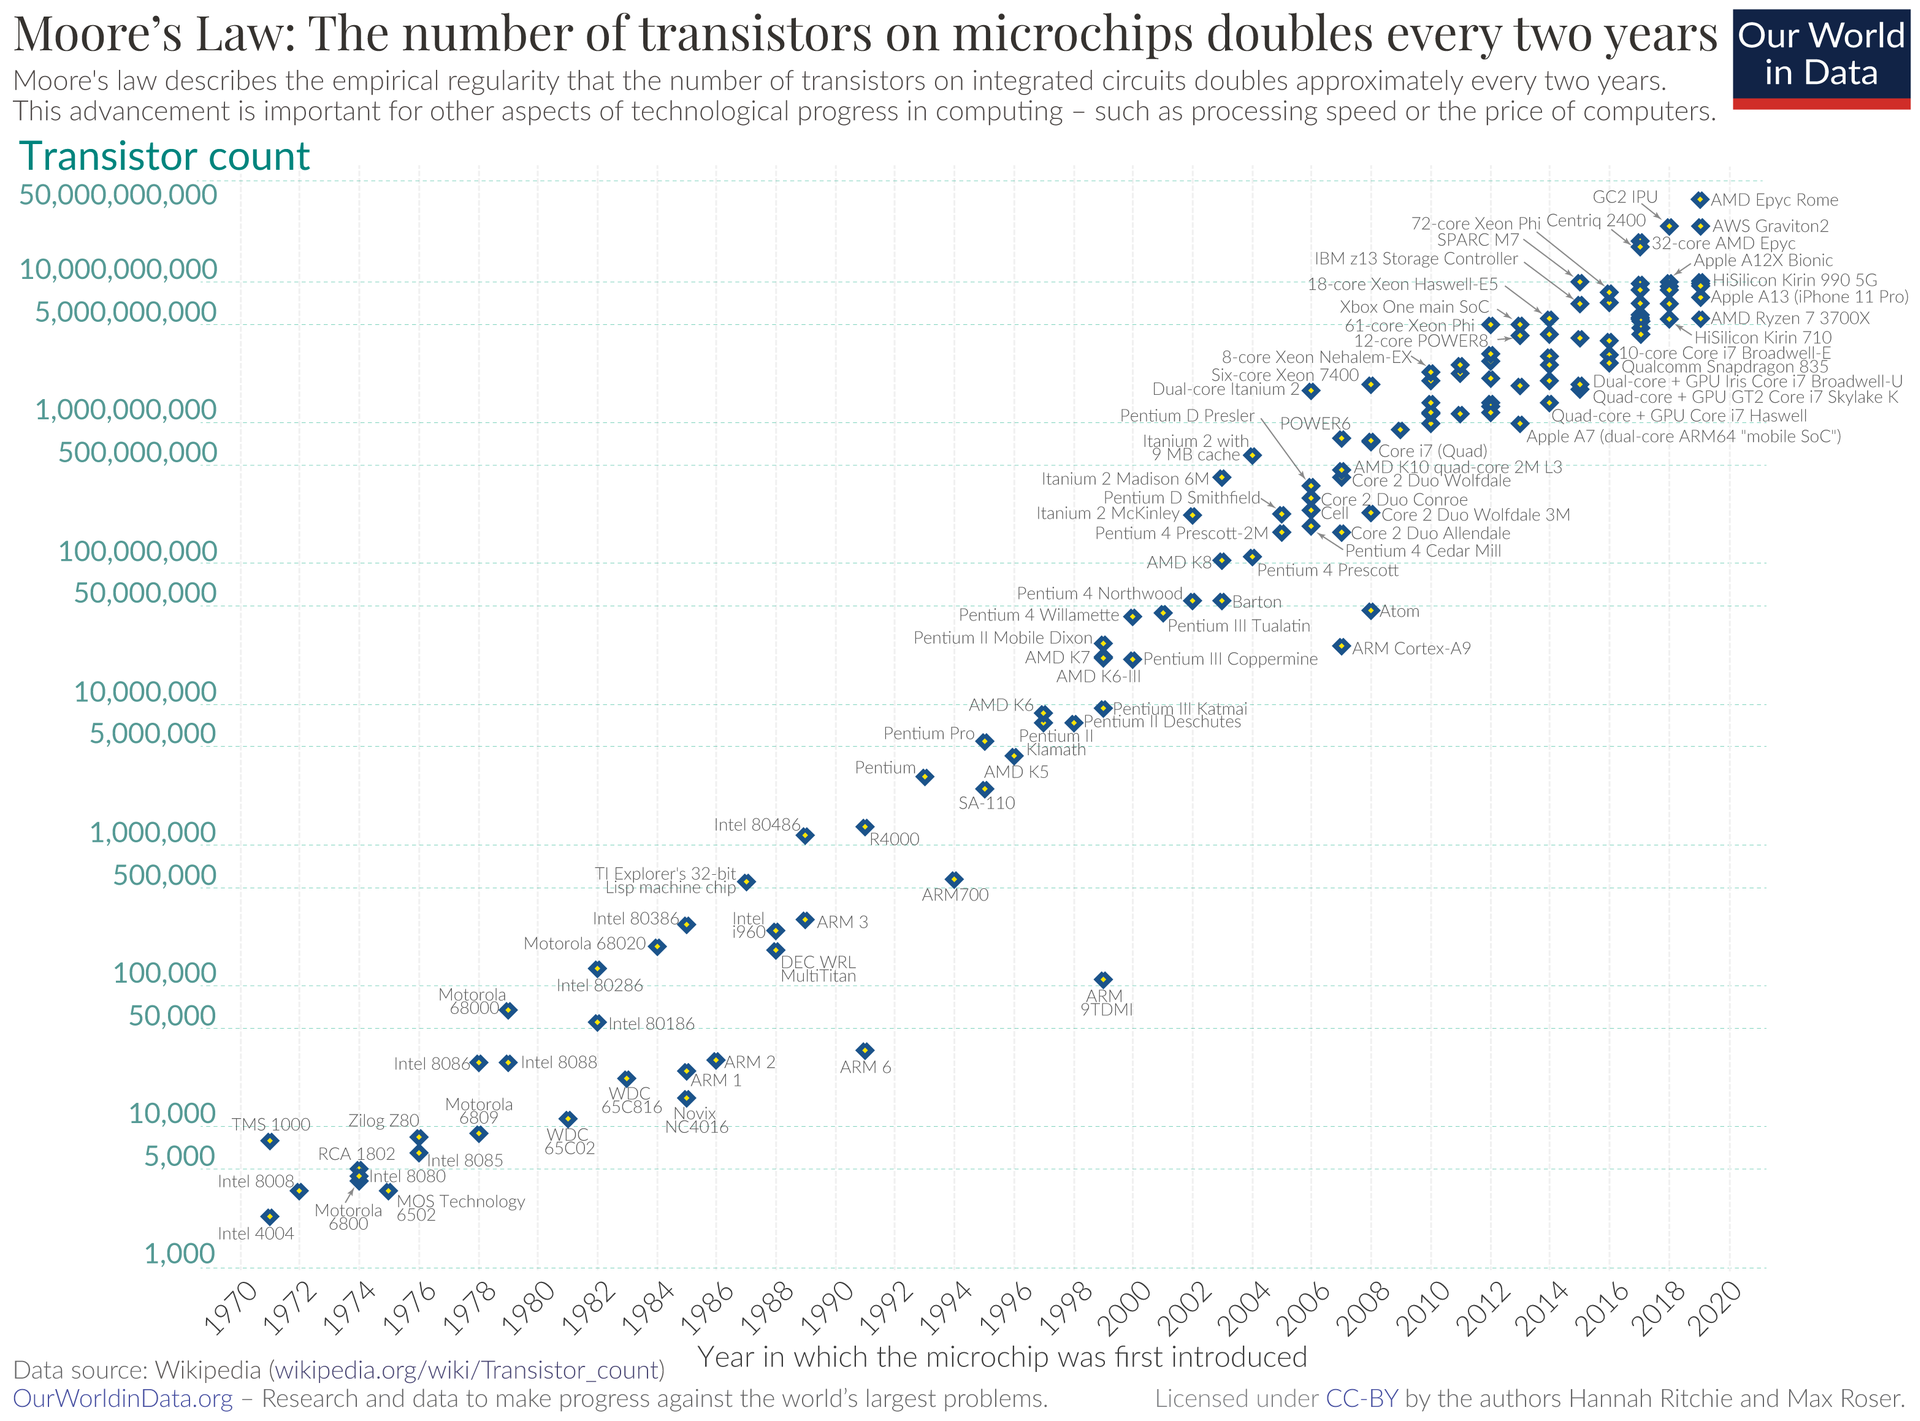
\includegraphics[width=1\linewidth]{img/ch1/moore15} \caption{Moores Law}\label{fig:fig115}
\end{figure}

Considering that graph above, one could be very optimistic. There does not seem to be any break in that trend. The best fit in these data points seems to be a straight line with constant slope. Since the scale on the vertical axis is logarithmic, this looks like exponential growth at a constant rate. If there were no extra information one could become quite sanguine and expect constant exponential technological progress to continue.

Alas, there are other things to consider. What did it take to maintain the incredible growth of computing power summarized by Moore's law?

\begin{figure}
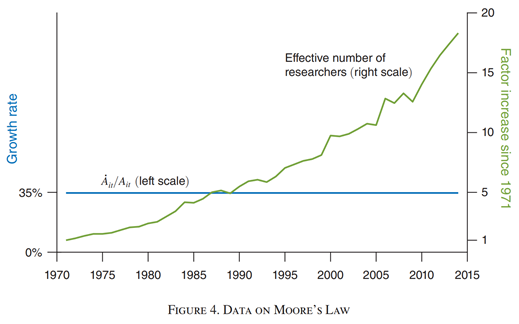
\includegraphics[width=1\linewidth]{img/ch1/moore16} \caption{Moore’s law requires huge increases in the number of researchers}\label{fig:fig116}
\end{figure}

Figure \ref{fig:fig116} shows that over time the number of workers/scientists required to maintain Moore's law want up by a factor of 25 over that period.

A factor of 25!

We can conclude from these two numbers that back in the 1970s, it was easier to double every two years. Now it is harder to double. It takes more resources to double.

That is diminishing returns.

There is no hint in the data, these two series in Figures 3 and 4, that future doubling will require fewer inputs.

We picked the low hanging fruit first. Now we got to climb higher.

Figure \ref{fig:fig117} shows something similar for agriculture: Yields per acre have been growing, but at declining rates but the number of researchers has been rising tremendously. Wheat, corn, soybeans, cotton; its all the same story.

\begin{figure}
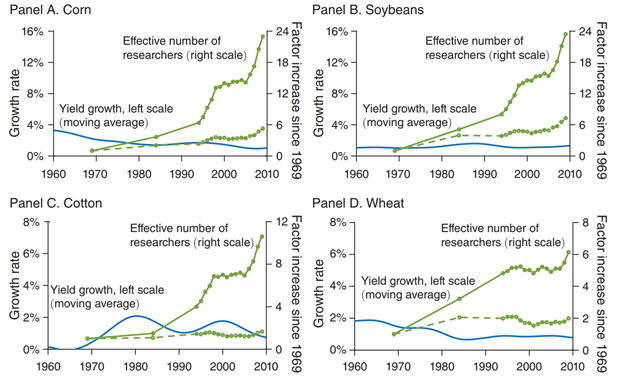
\includegraphics[width=1\linewidth]{img/ch1/moore17} \caption{For agriculture it seems the same holds true. Increases in productivity come at an ever increasing resource requirement.}\label{fig:fig117}
\end{figure}

Low hanging fruit was picked long time ago.

Figure \ref{fig:fig118} panel b shows the same story for mortality or survival from breast cancer. Mortality rates are way down, and they are declining, albeit at declining rates. Research effort measured by scientific publications and clinical trials are way up.

\begin{figure}
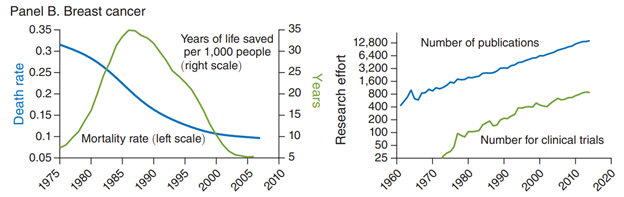
\includegraphics[width=1\linewidth]{img/ch1/moore18} \caption{For health again it seems the same holds true. Increasing productivity comes at the cost of ever increasing resource requirements.}\label{fig:fig118}
\end{figure}

Same old song: Low hanging fruit was picked years ago.

Figure \ref{fig:fig119} shows how drastic these diminishing returns are. Peak productivity was reached around 1990 when one clinical trial was responsible for about 16 life years saved per 100,000. Now we are down to 1.

A drop from 16 to 1.

\begin{figure}
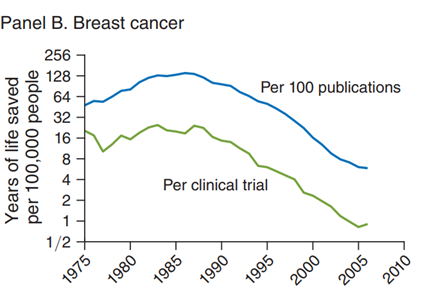
\includegraphics[width=1\linewidth]{img/ch1/moore19} \caption{sample caption}\label{fig:fig119}
\end{figure}

Most low hanging fruit seems to be gone. If we want to get any fruit, we got to climb REEEEAAAAAALLLLLLY high.

Since there seem to be many industries where technological progress is only achieved with the help of ever-increasing numbers of scientists it is a fair question to ask whether this is true also in the aggregate, i.e., for the total economy.

The answer to this question is a resounding YES. Figure 1 shoes aggregate technological progress for the US economy over a 70-year period starting with the 1930s. The pattern is clear: There is no increase at all in the rate at which technology has progressed. If anything, there is a declining trend.

\begin{figure}
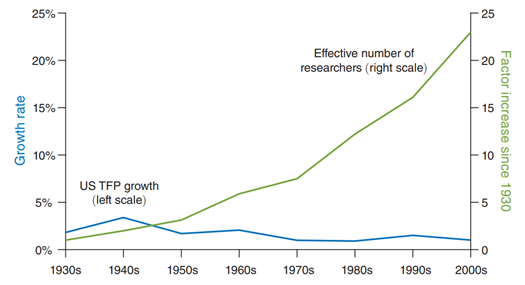
\includegraphics[width=1\linewidth]{img/ch1/moore20} \caption{sample caption}\label{fig:fig120}
\end{figure}

Figure \ref{fig:fig120} shows that this rise in productivity (at a declining rate) has been accomplished by an increase in researchers in the order of a factor of 20! This is huge.

Just like at the level of individual industries or activities, there is no evidence that these trends will be reversed. We can, with some degree of confidence predict, that future economic growth will be lower than past economic growth.

Those politicians running for election, who promise to make the economy grow at 3 or 4 \% annually, have to work really hard to fulfill their promises, since they are working against strong headwinds that are basically beyond their control.

(All the above figures are from the first paper listed below.)

The second paper below addresses the questions:
- What factors are contributors to the growth of real per capita GDP or output for short? And how important are they?
- What factors are contributors to technological progress or the growth in productivity? And how important are they?

Given the production function specified above, we can decompose the growth in output into the following components
1. Changes in the ratio of capital to output
2. Changes in educational attainment/ growth in human capital
3. Changes in the employment to population ratio
4. Changes in the fraction of workers in production rather than research.

Given the production function for new ideas we can decompose the growth rate of new ideas above we can decompose the rate of technological progress into:
- Changes in the fraction of workers employed in research rather than production
- Changes in the overall labor force.

How big is each of these factors? Jones (2021) provides the estimates. In the US starting in the 1950s, an increase in fraction of people employed is responsible for growth of 0.2\%, the increase in human capital per person is responsible for growth of 0.5 \% and technological progress contributes 1.3\% for a total of 2\% annual real per capita growth. Productivity growth or technological progress is responsible for the lion's share of growth.

Population growth contributes 0.3 \% to growth of productivity, while research intensity, hiring more researchers contributes 0.7 \% to productivity growth.

What is the potential for future economic growth?

It seems difficult to imagine that educational attainment can still increase substantially. In the US median years of schooling increased relatively rapidly till about 1980, but then the curve flattened out and that growth diminished. It is unlike that that growth will increase in the near term.

We are already hiring more and more researchers to generate more ideas with diminishing returns. Hiring more and more researchers comes at a cost of fewer workers in production with a corresponding current output decline. It seems hard to think of factors that can turn the declining research productivity around.

How about population growth? As the population grows, there are potentially more researchers as well. But population growth rates are falling worldwide?

Perhaps we can do a better job identifying and fostering future Einsteins and Curies? According to some estimates only 12\% of inventors are women, while roughly half of the population is women. Policies that increase that number might increase growth by 0.3\%.

\url{https://web.stanford.edu/~chadj/dignity.pdf}

\url{https://web.stanford.edu/~chadj/annualreview.pdf}

\hypertarget{appendix}{%
\chapter{Appendix}\label{appendix}}

In the appendix we dig more into concepts we gloss over in the text, however you may not be familiar with:

\begin{enumerate}
\def\labelenumi{\arabic{enumi}.}
\tightlist
\item
  Statistical Fundamentals

  \begin{enumerate}
  \def\labelenumii{\alph{enumii}.}
  \tightlist
  \item
    Percentiles
  \end{enumerate}
\end{enumerate}

\hypertarget{statistical-fundamentals}{%
\section{Statistical Fundamentals}\label{statistical-fundamentals}}

\hypertarget{percentiles}{%
\subsection{Percentiles}\label{percentiles}}

  \bibliography{book.bib,packages.bib}

\end{document}
